% TeX Live 2025 XeLaTeX
\documentclass[UTF8, 12pt, a4paper, oneside, onecolumn, fontset=none]{ctexart}
\usepackage{anyfontsize}
\usepackage{geometry}
\geometry{left=1.5cm, right=1.5cm, top=1.8cm, bottom=0.9cm}

\usepackage{unicode-math, mathrsfs, xcolor, inputenc}
\definecolor{pagecolor}{HTML}{C7EDCC}
\pagecolor{pagecolor}
\setCJKmainfont[AutoFakeBold, AutoFakeSlant]{LXGW WenKai}
\setCJKmonofont[AutoFakeBold, AutoFakeSlant]{MapleMono-CN-Regular}
\setCJKsansfont[AutoFakeBold, AutoFakeSlant]{LXGW WenKai}
\setmainfont[AutoFakeBold, AutoFakeSlant]{LXGW WenKai}
\setmonofont[AutoFakeBold, AutoFakeSlant]{MapleMono-CN-Regular}
\setsansfont[AutoFakeBold, AutoFakeSlant]{LXGW WenKai}
\setmathfont{Latin Modern Math}
\setmathrm{Latin Modern Math}

\usepackage{amsmath, amsthm, cases, graphicx, subfigure, tikz, caption, subcaption, siunitx, keyval, physics2}
\DeclareSIUnit\angstrom{Å}
\usephysicsmodule{ab, ab.braket}
\usepackage[version=4]{mhchem}
\usepackage[flushleft]{threeparttable}
\usepackage{hyperref, bookmark}
\hypersetup{colorlinks=true, urlcolor=blue, filecolor=blue, linkcolor=blue}
\usepackage[backend=biber, sorting=none]{biblatex}
\addbibresource{/Users/Linyan/Zotero/MyBibTeX.bib}

\ctexset{section={format=\bfseries\zihao{4}\flushleft}}
\renewcommand\thesubsection{\thesection.\arabic{subsection}}
\numberwithin{equation}{subsection}
\renewcommand\theequation{\thesubsection.\arabic{equation}}
\makeatletter
\renewcommand{\maketag@@@}[1]{\hbox{\m@th\normalsize\normalfont#1}}%
\makeatother
\usepackage{indentfirst}

\usepackage{listings}
\lstset{
      basicstyle      =    \zihao{-5}\ttfamily,
      numberstyle     =    \zihao{-5}\ttfamily,
      keywordstyle    =    \color{blue},
      keywordstyle    =    [2]\color{teal},
      stringstyle     =    \color{magenta},
      commentstyle    =    \color{red}\ttfamily,
      breaklines=true,     % 自动换行
      columns=fixed,       % 固定字间距
      flexiblecolumns,     % 别问为什么,加上这个
      numbers         =    left,% 行号的位置在左边
      showspaces      =    false,% 是否显示空格
      numberstyle     =    \zihao{-5}\ttfamily,% 行号的样式,小五号,tt 等宽字体
      showstringspaces=    false,
      captionpos      =    t,% 这段代码的名字所呈现的位置,t 指的是 top 上面
      frame           =    lrtb,% 显示边框
}

\lstdefinestyle{Python}{
      language        =    Python,
      basicstyle      =    \zihao{-5}\ttfamily,
      numberstyle     =    \zihao{-5}\ttfamily,
      keywordstyle    =    \color{blue},
      keywordstyle    =    [2]\color{teal},
      stringstyle     =    \color{magenta},
      commentstyle    =    \color{red}\ttfamily,
      breaklines      =    true,% 自动换行,建议不要写太长的行
      columns         =    fixed,% 如果不加这一句,字间距就不固定
      basewidth       =    0.5em,
}

\title{球面天文}
\author{林衍}
\date{\today}

\begin{document}
\maketitle
\subsection*{前言}
本文是南京大学天文与空间科学学院本科生课程《球面天文》讲义。根据《球面天文学》(夏一飞、黄天衣编著)增添删改而成。本课程主要研究,如何将各观测站点观测值,一步步修正到泛用的星表历元坐标。

\newpage
\tableofcontents

\newpage
\section{基本知识}
\subsection{球面三角与天球}
通过球心的平面截球面所得的截面是一个圆,叫做大圆。不通过球心的平面截球面所得的截面也是一个圆,叫做小圆。通过球面上不在同一直径两端的两个点,能作且只能作一个大圆。

垂直于球面上一已知圆的球直径的端点,叫做这个圆的极。极到圆上各点的角距都是相等的。两个大圆的夹角等于两个大圆的两极之间的大圆弧。

把球面上的三个点用三个大圆弧联结起来,所围成的图形叫做球面三角形。大圆弧为球面三角形的边,通常用 $a, b, c$ 表示;大圆弧所夹成的角为球面三角形的角,通常用 $A, B, C$ 表示。边的大小就是大圆弧的弧长;球面角的大小则是以球面角的顶点为极作大圆、球面角的边或其延长线在大圆上所截取的弧段的大小。

三个顶点的极线所构成的球面三角形,或者以三条边的极为顶点构成的球面三角形,被称为原球面三角形的极三角形。
\begin{figure}[!htp]
\centering
\tikzset{every picture/.style={line width=0.75pt}}
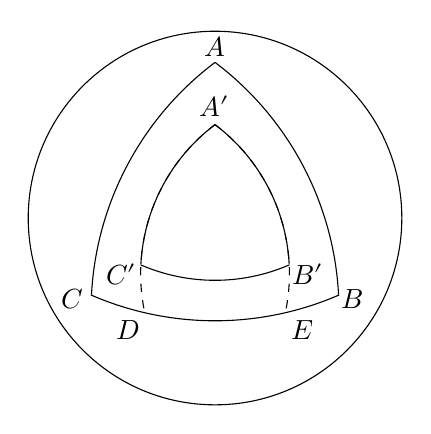
\begin{tikzpicture}[x=0.45pt, y=0.45pt, yscale=0.5, xscale=0.5]
% 天球
\draw (300, 0) arc(0:360:300);
% 大三角形
\draw (0, 250) arc(53:3:500);
\draw (0, 250) arc(127:177:500);
\draw (0,-165) arc(270:293.5:500);
\draw (0,-165) arc(270:246.5:500);
% 小三角形
\draw (0, 150) arc(53:3:300);
\draw [dashed](0, 150) arc(53:-12:300);
\draw (0, 150) arc(127:177:300);
\draw [dashed](0, 150) arc(127:192:300);
\draw (0,-100) arc(270:293.5:300);
\draw (0,-100) arc(270:246.5:300);
%Text
\draw (0, 275) node {$A$};
\draw (220,-130) node {$B$};
\draw (-230,-130) node {$C$};
\draw (-140,-180) node {$D$};
\draw (140,-180) node {$E$};
\draw (0, 180) node {$A'$};
\draw (150,-90) node {$B'$};
\draw (-150,-90) node {$C'$};
\end{tikzpicture}
\captionsetup{justification=raggedright, singlelinecheck=false}
\caption{球面三角形 $ABC$ 和其对应的极三角形 $A'B'C'$.}
\end{figure}

考虑转动球面,直到 $\overset{\frown}{AB}$ 都位于纸面上,以 $A$ 为极作大圆,大圆垂直纸面,$B$ 同理。两个大圆交点为 $C'$ 点,$C'$ 和球心的连线垂直纸面,因此 $C'$ 到 $\overset{\frown}{AB}$ 上的点距离都为 $\ang{90;;}, C'$ 是 $\overset{\frown}{AB}$ 的极。按同样方法可作出 $B', A'$. 因为 $C', B'$ 到 $A$ 的距离都是 $\ang{90;;}$, 所以 $C', B'$ 在以 $A$ 为极的大圆上。根据大圆弧定义可知 $\overset{\frown}{C'B'}$ 的极就是 $A$. 因此两个三角形互为极三角形,按两种方法定义出的极三角形是同一个。

若是延长 $A'C', A'B'$ 交 $\overset{\frown}{BC}$ 于 $D, E$ 点,根据球面角和极三角形定义可知 $\angle{A'}=\overset{\frown}{DE}$, 且 $\overset{\frown}{CD}+\overset{\frown}{DE}=\ang{90;;},\overset{\frown}{DE}+\overset{\frown}{EB}=\ang{90;;}$, 因此 $\angle{A'}+\overset{\frown}{BC}=\ang{180;;}$, 极三角形对应边角互补。这是一个很有用的性质,这意味着球面三角公式中边角某种意义上是等价的。

天球是一单位圆。在天球上按一定的原则选取某一点为极,称为第一极,与之相对的一点被称为第二极,对应的大圆是基本圈。根据定义基本圈的夹角等于第一极之间的大圆弧,如北黄极和北天极间的夹角就等于黄赤交角。

如图\ref{天球与直角坐标系。}所示,基本圈上选择一点作为零点,经过零点和两极的大圆称为零经圈。零经圈与天体经圈的夹角为 $\mu$, 天体到第一极的极距为 $\ang{90;;}-\nu$. 称 $\mu,\nu$ 分别为经角和纬角。那么天体方向的单位矢量、天体的球面坐标 $\left(\mu,\nu\right)$ 与直角坐标 $\left(x, y, z\right)$ 之间的关系为
\begin{equation}
\vec{S}\left(\mu,\nu\right)=
\begin{pmatrix}
\cos{\mu}\cos{\nu}\\
\sin{\mu}\cos{\nu}\\
\sin{\nu}
\end{pmatrix}=
\begin{pmatrix}
x\\y\\z
\end{pmatrix}.
\end{equation}
如此一来,要研究天体运动既可以解球面三角形,也可以在直角坐标系中解矢量形式。

值得注意的是,研究天体运动时经常要作垂直于极轴的小圆。大圆的半径是单位一,小圆的半径往往是 $\cos{\nu}$, 这在第六章自行的分析中尤为重要。

\begin{figure}[!htp]
\centering
\tikzset{every picture/.style={line width=0.75pt}}
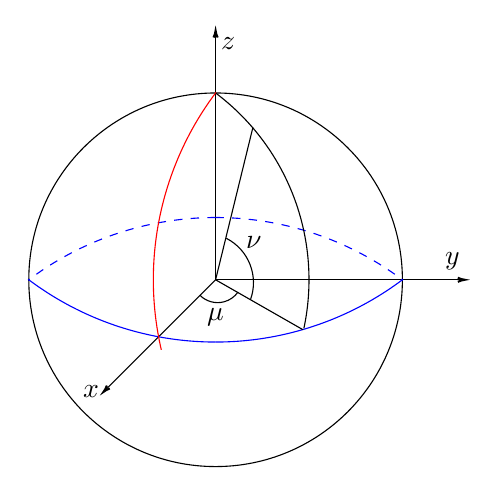
\begin{tikzpicture}[x=0.45pt, y=0.45pt, yscale=0.5, xscale=0.5]
% 天球
\draw (300, 0) arc(0:360:300);
\draw (0, 0) -- (400, 0);
\draw [shift={(400, 0)}, rotate=180][line width=0.75](10.93,-3.29) .. controls (6.95,-1.4) and (3.31,-0.3) .. (0, 0) .. controls (3.31, 0.3) and (6.95, 1.4) .. (10.93, 3.29); 
\draw (0, 0) -- (0, 400);
\draw [shift={(0, 400)}, rotate = -90] [color={rgb, 255: red, 0; green, 0; blue, 0 }  ][line width=0.75]    (10.93,-3.29) .. controls (6.95,-1.4) and (3.31,-0.3) .. (0, 0) .. controls (3.31, 0.3) and (6.95, 1.4) .. (10.93, 3.29);
\draw (0, 0) -- (-180,-180);
\draw [shift={(-180,-180)}, rotate = 45][line width=0.75](10.93,-3.29) .. controls (6.95,-1.4) and (3.31,-0.3) .. (0, 0) .. controls (3.31, 0.3) and (6.95, 1.4) .. (10.93, 3.29);
% 基本圈
\draw [blue](0,-100) arc(270:307:500);
\draw [blue](0,-100) arc(270:233:500);
\draw [blue][dashed](0, 100) arc(90:127:500);
\draw [blue][dashed](0, 100) arc(90:53:500);
\draw [red](-100, 0) arc(180:143:500);
\draw [red](-100, 0) arc(180:193:500);
\draw (150, 0) arc(0:53:375);
\draw (150, 0) arc(0:-12:375);
\draw (0, 0) -- (140,-80);
\draw (0, 0) -- (60, 245);
\draw (-25,-25) arc(225:325:40);
\draw (56,-32) arc(-20:63:80);
%Text
\draw (20, 380) node {$z$};
\draw (380, 30) node {$y$};
\draw (-200,-180) node {$x$};
\draw (0,-60) node {$\mu$};
\draw (60, 60) node {$\nu$};
\draw (-80,-150) node {零点};
\draw (-110, 200) node {\textcolor{red}{零经圈}};
\draw (-190,-30) node {\textcolor{blue}{基本圈}};
\draw (80, 330) node {第一极};
\end{tikzpicture}
\captionsetup{justification=raggedright, singlelinecheck=false}
\caption{天球与直角坐标系。}
\label{天球与直角坐标系。}
\end{figure}

解球面三角需要一些基本公式。为了方便地推导公式,同时为了方便地进行坐标系转换,引入坐标变换矩阵,分为坐标轴反向变换矩阵和旋转矩阵两类。

坐标轴反向变换矩阵一般用来变换左手系和右手系,
\begin{equation}
P_{X}=
\begin{pmatrix}
-1 & 0 & 0\\
0 & 1 & 0\\
0 & 0 & 1\\
\end{pmatrix},
P_{Y}=
\begin{pmatrix}
1 & 0 & 0\\
0 & -1 & 0\\
0 & 0 & 1\\
\end{pmatrix},
P_{Z}=
\begin{pmatrix}
1 & 0 & 0\\
0 & 1 & 0\\
0 & 0 & -1\\
\end{pmatrix}.
\end{equation}

右手系中,若角度在 $x\text{\textendash}y$ 平面增长,若角速度矢量指向 $z$ 轴正方向则称角度在正方向增加。注意左手系中用左手判断角速度矢量方向,因此坐标轴旋转矩阵仅有三种:
\begin{equation}
R_{X}\left(\theta\right)=
\begin{pmatrix}
1 & 0 & 0\\
0 & \cos{\theta} & \sin{\theta}\\
0 & -\sin{\theta} & \cos{\theta}\\
\end{pmatrix},
R_{Y}\left(\theta\right)=
\begin{pmatrix}
\cos{\theta} & 0 & -\sin{\theta}\\
0 & 1 & 0\\
\sin{\theta} & 0 & \cos{\theta}\\
\end{pmatrix},
R_{Z}\left(\theta\right)=
\begin{pmatrix}
\cos{\theta} & \sin{\theta} & 0\\
-\sin{\theta} & \cos{\theta} & 0\\
0 & 0 & 1
\end{pmatrix}.
\end{equation}

注意几个有趣的结论:
\begin{align}
R^{-1}\left(\theta\right)&=R\left(-\theta\right)=R^{\top}\left(\theta\right).\\
P_{X}R_{X}\left(\theta\right)P_{X}&=R_{X}\left(\theta\right).\\
P_{Y}R_{X}\left(\theta\right)P_{Y}&=R_{X}\left(-\theta\right).
\end{align}

现在可以进行基本公式推导了。考虑一个球面三角形 $\Delta{}ABC$, 以原点和 $\overset{\frown}{AB}$ 的极连线方向为 $y, y'$ 轴,以 $OA$ 为 $z$ 轴,以 $OB$ 为 $z'$ 轴建立两个直角坐标系。如图\ref{基本公式证明。}所示,在直角坐标系 $x\text{\textendash}y\text{\textendash}z$ 中,$C$ 的天球方向单位矢量为 $\vec{S}\left(A,\ang{90;;}-b\right)$, 而在直角坐标系 $x'\text{\textendash}y'\text{\textendash}z'$ 中,$C$ 的天球方向单位矢量为 $\vec{S}\left(\ang{180;;}-B,\ang{90;;}-a\right)$. 转换到直角坐标,并考虑第二个坐标系是第一个坐标系绕 $y$ 轴正向旋转 $c$, 因此有
\begin{equation}
\begin{pmatrix}
-\cos{B}\sin{a}\\
\sin{B}\sin{a}\\
\cos{a}
\end{pmatrix}=
\begin{pmatrix}
\cos{c} & 0 & -\sin{c}\\
0 & 1 & 0\\
\sin{c} & 0 & \cos{c}\\
\end{pmatrix}
\begin{pmatrix}
\cos{A}\sin{b}\\
\sin{A}\sin{b}\\
\cos{b}
\end{pmatrix}.
\end{equation}

\begin{figure}[!htp]
\centering
\tikzset{every picture/.style={line width=0.75pt}}
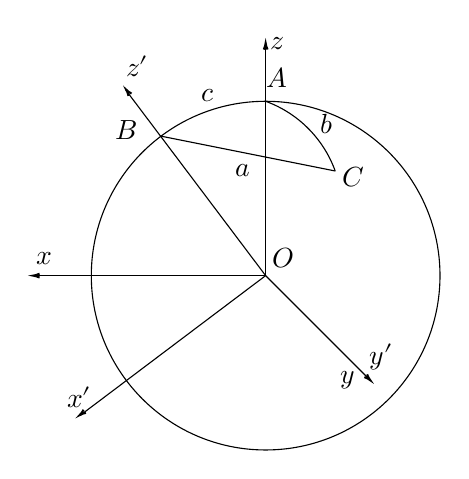
\begin{tikzpicture}[x=0.42pt, y=0.42pt, yscale=0.5, xscale=0.5]
% 天球
\draw (300, 0) arc(0:360:300);
%x
\draw (0, 0) -- (-400, 0);
\draw [shift={(-400, 0)}, rotate=0][line width=0.75](10.93,-3.29) .. controls (6.95,-1.4) and (3.31,-0.3) .. (0, 0) .. controls (3.31, 0.3) and (6.95, 1.4) .. (10.93, 3.29); 
\draw [shift={(0, 0)}, rotate=37](0, 0) -- (-400, 0);
\draw [shift={(-320,-240)}, rotate=37][line width=0.75](10.93,-3.29) .. controls (6.95,-1.4) and (3.31,-0.3) .. (0, 0) .. controls (3.31, 0.3) and (6.95, 1.4) .. (10.93, 3.29); 
%z
\draw (0, 0) -- (0, 400);
\draw [shift={(0, 400)}, rotate = -90] [color={rgb, 255: red, 0; green, 0; blue, 0 }  ][line width=0.75]    (10.93,-3.29) .. controls (6.95,-1.4) and (3.31,-0.3) .. (0, 0) .. controls (3.31, 0.3) and (6.95, 1.4) .. (10.93, 3.29);
\draw [shift={(0, 0)}, rotate = 37](0, 0) -- (0, 400);
\draw [shift={(-240, 320)}, rotate = -53] [color={rgb, 255: red, 0; green, 0; blue, 0 }  ][line width=0.75]    (10.93,-3.29) .. controls (6.95,-1.4) and (3.31,-0.3) .. (0, 0) .. controls (3.31, 0.3) and (6.95, 1.4) .. (10.93, 3.29);
%y
\draw (0, 0) -- (180,-180);
\draw [shift={(180,-180)}, rotate = 135][line width=0.75](10.93,-3.29) .. controls (6.95,-1.4) and (3.31,-0.3) .. (0, 0) .. controls (3.31, 0.3) and (6.95, 1.4) .. (10.93, 3.29);
% 三角形
\draw (0, 300) arc(70:20:200);
\draw (-180, 240) -- (120, 180);
%Text
\draw (20, 400) node {$z$};
\draw (-220, 360) node {$z'$};
\draw (-380, 30) node {$x$};
\draw (-320,-210) node {$x'$};
\draw (200,-140) node {$y'$};
\draw (140,-180) node {$y$};
\draw (20, 340) node {$A$};
\draw (-240, 250) node {$B$};
\draw (150, 170) node {$C$};
\draw (-40, 180) node {$a$};
\draw (105, 260) node {$b$};
\draw (-100, 310) node {$c$};
\draw (30, 30) node {$O$};
\end{tikzpicture}
\captionsetup{justification=raggedright, singlelinecheck=false}
\caption{基本公式证明。}
\label{基本公式证明。}
\end{figure}

整理得到
\begin{align}
-\cos{B}\sin{a}&=\cos{c}\cos{A}\sin{b}-\sin{c}\cos{b}.\label{1.1.8}\\
\sin{B}\sin{a}&=\sin{A}\sin{b}.\label{1.1.9}\\
\cos{a}&=\sin{c}\cos{A}\sin{b}+\cos{c}\cos{b}.\label{1.1.10}
\end{align}
其中 (\ref{1.1.9}) 式为正弦公式,(\ref{1.1.10}) 式为边余弦公式,(\ref{1.1.8}) 式为第一五元素公式。边余弦公式和第一五元素公式考虑极三角形边角互补并去掉角标,分别得到角余弦公式和第二五元素公式:
\begin{align}
\cos{A}&=\sin{C}\cos{a}\sin{B}-\cos{B}\cos{C}.\\
\cos{b}\sin{A}&=\cos{C}\cos{a}\sin{B}+\sin{C}\cos{b}.\label{1.1.12}
\end{align}
(\ref{1.1.12}) 式结合正弦公式得到四元素公式:
\begin{align}
\frac{\cos{b}\sin{A}}{\sin{B}}&=\cos{C}\cos{a}+\sin{C}\frac{\cos{b}}{\sin{B}}.\notag\\
\sin{a}\cot{b}&=\cos{C}\cos{a}+\sin{c}\cot{b}.
\end{align}

\subsection{恒星位移公式}
考虑大气折射、周日视差、周日光行差、周年视差、周年光行差、岁差、章动、恒星自行等因素,恒星在天球上的位置会发生改变。对这些因素一步步进行修正,便是球面天文的主要工作。恒星位移总是处于穿过恒星和某一固定点 $A$ ($A$ 被称作向点)的大圆上。
\begin{figure}[!htp]
\centering
\tikzset{every picture/.style={line width=0.75pt}}
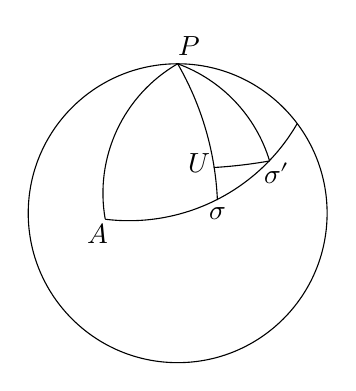
\begin{tikzpicture}[x=0.36pt, y=0.36pt, yscale=0.5, xscale=0.5]
% 天球
\draw (300, 0) arc(0:360:300);
% 三角形
\draw (0, 300) arc(120:190:300);
\draw (240, 180) arc(-30:-97:390);
\draw (0, 300) arc(70:17:300);
\draw (0, 300) arc(30:2.5:600);
\draw (185, 105) arc(280:273.5:1000);
%Text
\draw (20, 335) node {$P$};
\draw (-160,-40) node {$A$};
\draw (80, 0) node {$\sigma$};
\draw (200, 80) node {$\sigma'$};
\draw (40, 100) node {$U$};
\end{tikzpicture}
\captionsetup{justification=raggedright, singlelinecheck=false}
\caption{恒星位移示意图。}
\label{恒星位移示意图。}
\end{figure}

\subsubsection{球面三角方法}
图\ref{恒星位移示意图。}中记
\begin{equation}
A=\left(\alpha_{0},\delta_{0}\right),\sigma=\left(\alpha,\delta\right),\sigma'=\left(\alpha',\delta'\right),
\end{equation}
然后以 $P$ 为极过 $\sigma'$ 作小圆弧 $\overset{\frown}{U\sigma'}$ 交 $\overset{\frown}{P\sigma}$ 于 $U$, 显然
\begin{equation}
\overset{\frown}{U\sigma}=\delta'-\delta{},\overset{\frown}{U\sigma'}=\left(\alpha'-\alpha\right)\cos{\delta'}.
\end{equation}
由于恒星位移是个很小的量,因此球面三角形 $\Delta{}U\sigma\sigma'$ 可近似看作平面直角三角形,有
\begin{equation}
\delta'-\delta=\overset{\frown}{\sigma\sigma'}\cos{\angle{P\sigma\sigma'}},\left(\alpha'-\alpha\right)\cos{\delta'}=\overset{\frown}{\sigma\sigma'}\sin{\angle{P\sigma\sigma'}}.
\end{equation}
我们可以记
\begin{equation}
\overset{\frown}{\sigma\sigma'}=k\sin{\overset{\frown}{A\sigma}},
\end{equation}
其中恒星位移远离向点 $A$ 时 $k$ 取正值。现在要得到恒星位移我们需要知道 $\cos{\angle{P\sigma\sigma'}}\sin{\overset{\frown}{A\sigma}}$ 和 $\sin{\angle{P\sigma\sigma'}}\sin{\overset{\frown}{A\sigma}}$ 的取值。而在 $\Delta{}PA\sigma$ 中
\begin{equation}
\angle{AP\sigma}=\alpha-\alpha_{0},\overset{\frown}{PA}=\ang{90;;}-\delta{}_{0},\overset{\frown}{P\sigma}=\ang{90;;}-\delta{},
\end{equation}
应用正弦和第一五元素公式得到
\begin{align}
\frac{\sin{\overset{\frown}{A\sigma}}}{\sin{\angle{AP\sigma}}}&=\frac{\sin{\overset{\frown}{AP}}}{\sin{\angle{A\sigma P}}}=\frac{\sin{\overset{\frown}{AP}}}{\sin{\angle{P\sigma\sigma'}}},\\
\sin{\overset{\frown}{A\sigma}}\cos{\angle{A\sigma{}P}}&=\sin{\overset{\frown}{P\sigma}}\cos{\overset{\frown}{PA}}-\cos{\overset{\frown}{P\sigma}}\cos{\angle{AP\sigma}}\sin{\overset{\frown}{PA}}.
\end{align}
如此一来
\begin{align}
\cos{\angle{P\sigma\sigma'}}\sin{\overset{\frown}{A\sigma}}=-\sin{\overset{\frown}{A\sigma}}\cos{\angle{A\sigma P}}&=-\sin{\overset{\frown}{P\sigma}}\cos{\overset{\frown}{PA}}+\cos{\overset{\frown}{P\sigma}}\cos{\angle{AP\sigma}}\sin{\overset{\frown}{PA}}\notag\\
&=\sin{\delta}\cos{\left(\alpha-\alpha_{0}\right)}\cos{\delta_{0}}-\cos{\delta}\sin{\delta_{0}}.\\
\sin{\angle{P\sigma\sigma'}}\sin{\overset{\frown}{A\sigma}}=\sin{\overset{\frown}{AP}}\sin{\angle{AP\sigma}}&=\cos{\delta{}_{0}}\sin{\left(\alpha-\alpha_{0}\right)}.
\end{align}
由于恒星位移是个小量,我们可认为 $\cos{\delta'}=\cos{\delta}$, 最后得到
\begin{align}
\alpha'-\alpha&=k\sec{\delta{}}\cos{\delta{}_{0}}\sin{\left(\alpha-\alpha_{0}\right)},\label{1.2.10}\\
\delta'-\delta{}&=k\left[\sin{\delta}\cos{\left(\alpha-\alpha_{0}\right)}\cos{\delta{}_{0}}-\cos{\delta{}}\sin{\delta{}_{0}}\right].\label{1.2.11}
\end{align}

\subsubsection{矢量方法}
考虑三个天体方向单位矢量
\begin{align}
\vec{S}_{0}=A\left(\alpha_{0},\delta{}_{0}\right),\vec{S}=\sigma\left(\alpha,\delta{}\right),\vec{S}'=\sigma'\left(\alpha',\delta'\right),
\end{align}
并且记
\begin{equation}
\overset{\frown}{A\sigma}=\theta,\overset{\frown}{\sigma\sigma'}=\symup{d}\theta,\symup{d}\theta=k\sin{\theta}.
\end{equation}
再引入两个辅助矢量 $\vec{a}=\left\vert{}\vec{a}\right\vert{}\vec{S}_{0},\vec{b}=\left\vert{}\vec{b}\right\vert{}\vec{S},\vec{S}'-\vec{S}=\vec{b}-\vec{a}$.
\begin{figure}[!htp]
\centering
\tikzset{every picture/.style={line width=0.75pt}}
\begin{tikzpicture}[x=0.4pt, y=0.4pt, yscale=1, xscale=1]
\draw (0, 0) -- (100, 240);
\draw [shift={(100, 240)}, rotate=248][line width=0.75](10.93,-3.29) .. controls (6.95,-1.4) and (3.31,-0.3) .. (0, 0) .. controls (3.31, 0.3) and (6.95, 1.4) .. (10.93, 3.29); 
\draw (100, 240) -- (108.33, 260);
\draw [shift={(108.33, 260)}, rotate=248][line width=0.75](10.93,-3.29) .. controls (6.95,-1.4) and (3.31,-0.3) .. (0, 0) .. controls (3.31, 0.3) and (6.95, 1.4) .. (10.93, 3.29); 
\draw (0, 260) -- (108.33, 260);
\draw [shift={(108.33, 260)}, rotate=180][line width=0.75](10.93,-3.29) .. controls (6.95,-1.4) and (3.31,-0.3) .. (0, 0) .. controls (3.31, 0.3) and (6.95, 1.4) .. (10.93, 3.29); 
\draw (0, 0) -- (260, 0);
\draw [shift={(260, 0)}, rotate=180][line width=0.75](10.93,-3.29) .. controls (6.95,-1.4) and (3.31,-0.3) .. (0, 0) .. controls (3.31, 0.3) and (6.95, 1.4) .. (10.93, 3.29); 
\draw (0, 0) -- (0, 260);
\draw [shift={(0, 260)}, rotate=270][line width=0.75](10.93,-3.29) .. controls (6.95,-1.4) and (3.31,-0.3) .. (0, 0) .. controls (3.31, 0.3) and (6.95, 1.4) .. (10.93, 3.29);
\draw (100, 240) -- (0, 260);
\draw [shift={(0, 260)}, rotate=-12][line width=0.75](10.93,-3.29) .. controls (6.95,-1.4) and (3.31,-0.3) .. (0, 0) .. controls (3.31, 0.3) and (6.95, 1.4) .. (10.93, 3.29); 
\draw (0, 30) arc(90:68:30);
\draw (20, 0) arc(0:68:20);
%Text
\draw (-20, 0) node [anchor=north west][inner sep=0.75pt]   [align=left] {$O$};
\draw (80, 180) node [anchor=north west][inner sep=0.75pt]   [align=left] {$\vec{S}$};
\draw (280, 20) node [anchor=north west][inner sep=0.75pt]   [align=left] {$\vec{S}_{0}$};
\draw (-40, 200) node [anchor=north west][inner sep=0.75pt]   [align=left] {$\vec{S}'$};
\draw (40, 300) node [anchor=north west][inner sep=0.75pt]   [align=left] {$\vec{a}$};
\draw (120, 260) node [anchor=north west][inner sep=0.75pt]   [align=left] {$\vec{b}$};
\draw (-2, 93) node [anchor=north west][inner sep=0.75pt]   [align=left] {$\symup{d}\theta$};
\draw (30, 40) node [anchor=north west][inner sep=0.75pt]   [align=left] {$\theta$};
\end{tikzpicture}
\captionsetup{justification=raggedright, singlelinecheck=false}
\caption{天体方向单位矢量示意图。}
\label{天体方向单位矢量示意图。}
\end{figure}

如图\ref{天体方向单位矢量示意图。}所示,$\vec{a}$ 正对角为 $\ang{90;;}+\dfrac{\symup{d}\theta}{2}, \vec{b}$ 正对角为 $\ang{90;;}-\theta-\dfrac{\symup{d}\theta}{2}$, 运用平面三角正弦公式,得到
\begin{align}
\left\vert{}\vec{a}\right\vert{}&=\left\vert{}\vec{S}'-\vec{S}\right\vert{}\cos{\frac{\symup{d}\theta}{2}}/\sin{\theta},\\
\left\vert{}\vec{b}\right\vert{}&=\left\vert{}\vec{S}'-\vec S\right\vert{}\cos{\left(\theta+\frac{\symup{d}\theta}{2}\right)}/\sin{\theta}.
\end{align}
由于
\begin{equation}
\left\vert{}\vec{S}'-\vec S\right\vert{}=2\sin{\frac{\symup{d}\theta}{2}},
\end{equation}
直接得到
\begin{equation}
\vec{b}-\vec{a}=\vec{S}'-\vec{S}=\frac{2\sin{\dfrac{\symup{d}\theta}{2}}}{\sin{\theta}}\left[\cos{\left(\theta+\frac{\symup{d}\theta}{2}\right)}\vec{S}-\cos{\frac{\symup{d}\theta}{2}}\vec{S}_{0}\right].
\end{equation}
保留到小角的一阶量,上式变为
\begin{align}
\vec{S}'-\vec{S}&=\frac{\symup{d}\theta}{\sin{\theta}}\left(\cos{\theta}\cdot\vec{S}-\vec{S}_{0}\right)\notag\\
&=\frac{k\sin{\theta}}{\sin{\theta}}\vec{S}\times\left(\vec{S}\times\vec{S}_{0}\right)\notag\\
&=k\vec{S}\times\left(\vec{S}\times\vec{S}_{0}\right)=k\left[\vec{S}\left(\vec{S}\cdot\vec{S}_{0}\right)-\vec{S}_{0}\right].\label{1.2.18}
\end{align}
若采用赤道坐标系,(\ref{1.2.18}) 式就变为 (\ref{1.2.10}) 和 (\ref{1.2.11}) 式的形式。计算 $\symup{d}\alpha$ 和 $\symup{d}\delta{}$ 的具体方式为(一阶近似)
\begin{align}
\vec{S}&=\begin{pmatrix}
\cos{\alpha}\cos{\delta{}}\\
\sin{\alpha}\cos{\delta{}}\\
\sin{\delta{}}
\end{pmatrix},
\vec{S}_{0}=\begin{pmatrix}
\cos{\alpha_{0}}\cos{\delta_{0}}\\
\sin{\alpha_{0}}\cos{\delta_{0}}\\
\sin{\delta_{0}}
\end{pmatrix},\\
\vec{S}'-\vec{S}&=\symup{d}\vec{S}=\begin{pmatrix}
-\sin{\alpha}\cos{\delta}\symup{d}\alpha-\cos{\alpha}\sin{\delta}\symup{d}\delta\\
\cos{\alpha}\cos{\delta}\symup{d}\alpha-\sin{\alpha}\sin{\delta}\symup{d}\delta\\
\cos{\delta}\symup{d}\delta
\end{pmatrix}
=k\left[\vec{S}\left(\vec{S}\cdot\vec{S}_{0}\right)-\vec{S}_{0}\right].
\end{align}

若是不采用一阶近似,严格公式需要精确计算 $\tan{\left(\alpha'-\alpha\right)},\tan{\left(\delta'-\delta\right)}$ 等值,具体问题具体分析。第三章周日视差部分便采用了严格公式。

\subsection{天球坐标系}
\begin{table}[htbp]
\centering
\caption{天球坐标系。}
\begin{tabular}{c c c c c c c c}
\hline
坐标系 & 第一极 & 基本圈 & 经角零点 &  & 经角 & 纬角 & 余纬角\\
\cline{1-8}
地平 & 天顶 & 地平圈 & 北点或南点 & 左旋 & 方位角 $A$ & 高度角 $h$ & 天顶距 $z$\\
\cline{1-8}
时角 & 北天极 & 天赤道 & 上点 & 左旋 & 时角 $t$ & 赤纬 $\delta{}$ & 北极距 $p$\\
\cline{1-8}
赤道 & 北天极 & 天赤道 & 春分点 & 右旋 & 赤经 $\alpha$ & 赤纬 $\delta{}$ & 北极距 $p$\\
\cline{1-8}
黄道 & 北黄极 & 黄道 & 春分点 & 右旋 & 黄经 $\lambda$ & 黄纬 $\beta$ & 黄极距 $r$\\
\cline{1-8}
银道 & 北银极 & 银道 & 银心方向 & 右旋 & 银经 $l$ & 银纬 $b$ & \\
\cline{1-8}
\end{tabular}
\label{天球坐标系。}
\end{table}

由于我们已经介绍过第一极、第二极、基本圈、零经圈、零点、极距、左旋坐标系、右旋坐标系等概念,所以我们直接列出各种坐标系,如表\ref{天球坐标系。}所示。

地平坐标系中,天顶通过铅垂线确定,第二极被称作天底。北天极是地球自转轴通过地球北极延长后与天球的交点。通过天顶、天底、北天极的大圆被称作子午圈,它是地平系的零经圈。零经圈交地平圈于北点和南点,因此地平系经角是从北点或南点开始计量的。

很明显,天顶与观测站的地理坐标有关。如果掌握了观测时间以及一些恒星的地平坐标和赤道坐标,就可以根据球面三角给出天顶的赤道坐标,完成定位。

北天极和南天极将子午圈分成两个半圆,天体运行到上半子午圈的时候我们称天体上中天。

虽然实际观测中常用地平系来估计光污染和大气扰动,但由于不同观测者的天顶不同,以及地平坐标受地球自转影响而非线性变化,地平系不适合用来统一天体坐标。我们希望能找到一些坐标线性变化的天球系。这其实很简单,只要让地球自转的影响只体现在经角上就可以了,故采用北天极作为第一极。

天赤道是地球赤道面延伸后和天球相交得到的大圆。天赤道和子午圈相交得到的靠近南点的点被称作上点(或赤道最高点)。地球自西向东自转,等价于天球自东向西旋转,因此时角系是左旋的。很显然,时角衡量了天体上中天后又过去了多久。很自然地我们将一圈 $\ang{360;;}$ 划分为 $\qty{24}{h}$. 值得注意的是 $\ang{1;;}=\ang{;; 3600},\qty{1}{h}=\qty{3600}{s}$, 因此 $\ang{;; 15}=\qty{1}{s}$, 即每经过一秒钟天体时角就会改变 $\ang{;; 15}$. 我们立刻意识到,可以通过天体的位置来计时。

我们选择春分点作为时间计量的参考点。春分点是黄道对赤道的升交点(地球自西向东公转,反过来讲太阳周年运动也是自西向东,因此太阳周年视运动在天球上是逆时针的)。可以定义春分点连续两次上中天的时间间隔是恒星时中的 $\qty{24}{h}$, 春分点上中天的时刻是恒星时零点。当然由于太阳系其他天体对地球的引力摄动,春分点在天球上的位置实际上是不固定的,因此时间间隔和零点都会发生变化。

接着,选取春分点作为经角零点,我们可以定义赤道坐标系。易得上中天天体的赤经等于此刻春分点的时角,也就等于此刻的恒星时,等于任一天体赤经与其时角的和。地球上不同时区上中天天体赤经显然不同,因此恒星时是一种地方时。(反过来讲,如果排除时区影响我们也就可以确定一种“世界时”了。)

黄道坐标系没什么好讲的,或者说重要的部分我们将在第五章岁差章动部分展开。谈谈银道坐标系。银河系是个盘星系,其平均平面称为银河系对称面,通过太阳系质心且平行于银河系对称面的平面被称作银道面,它与天球相交得到的大圆是银道。虽然基本圈是银道,但零点并不是银道对天赤道的升交点 $N$, 而是银河系中心方向。因此我们可以这么考虑赤道到银道坐标系的变换:记 $N$ 赤经为 $\alpha_{N}$, 银经为 $l_{N}$, 银赤交角 $i$, 首先赤道系绕 $z$ 轴旋转 $\alpha_{N}$, 直到春分点 $\gamma$ 和 $N$ 重合,这样就可以绕 $x$ 轴旋转 $i$ 从而把基本圈从天赤道变成银道,最后再绕 $z$ 轴转动 $-l_{N}$ 从而把零点变为银河系中心。具体可如图\ref{银道坐标系。}所示。
\begin{equation}
\vec{S}\left(l, b\right)=R_{Z}\left(-l_{N}\right)R_{X}\left(i\right)R_{Z}\left(\alpha_{N}\right)\vec{S}\left(\alpha,\delta{}\right).
\end{equation}

\begin{figure}[!htp]
\centering
\tikzset{every picture/.style={line width=0.75pt}}
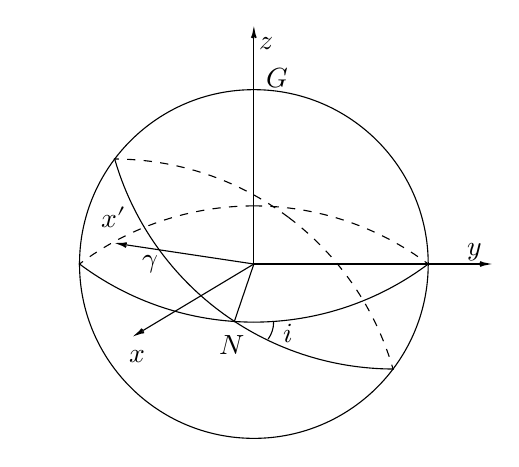
\begin{tikzpicture}[x=0.35pt, y=0.35pt, yscale=0.6, xscale=0.6]
% 天球
\draw (300, 0) arc(0:360:300);
\draw (0, 0) -- (400, 0);
\draw [shift={(400, 0)}, rotate=180][line width=0.75](10.93,-3.29) .. controls (6.95,-1.4) and (3.31,-0.3) .. (0, 0) .. controls (3.31, 0.3) and (6.95, 1.4) .. (10.93, 3.29); 
\draw (0, 0) -- (0, 400);
\draw [shift={(0, 400)}, rotate = -90] [color={rgb, 255: red, 0; green, 0; blue, 0 }  ][line width=0.75]    (10.93,-3.29) .. controls (6.95,-1.4) and (3.31,-0.3) .. (0, 0) .. controls (3.31, 0.3) and (6.95, 1.4) .. (10.93, 3.29);
\draw (0, 0) -- (-200,-120);
\draw [shift={(-200,-120)}, rotate = 30][line width=0.75](10.93,-3.29) .. controls (6.95,-1.4) and (3.31,-0.3) .. (0, 0) .. controls (3.31, 0.3) and (6.95, 1.4) .. (10.93, 3.29);
\draw (0, 0) -- (-230, 34.5);
\draw [shift={(-230, 34.5)}, rotate = -10][line width=0.75](10.93,-3.29) .. controls (6.95,-1.4) and (3.31,-0.3) .. (0, 0) .. controls (3.31, 0.3) and (6.95, 1.4) .. (10.93, 3.29);
% 基本圈
\draw (0,-100) arc(270:307:500);
\draw (0,-100) arc(270:233:500);
\draw (-60,-80) arc(233:270:500);
\draw (-60,-80) arc(233:196:500);
\draw [dashed](0, 100) arc(90:127:500);
\draw [dashed](0, 100) arc(90:53:500);
\draw [dashed](60, 80) arc(53:90:500);
\draw [dashed](60, 80) arc(53:16:500);
\draw (0, 0) -- (-34,-100);
\draw (34,-100) arc(0:-36:50);
%Text
\draw (20, 380) node {$z$};
\draw (380, 20) node {$y$};
\draw (-200,-160) node {$x$};
\draw (-240, 80) node {$x'$};
\draw (-40,-140) node {$N$};
\draw (60,-120) node {$i$};
\draw (-180, 0) node {$\gamma$};
\draw (-320, 200) node {天赤道};
\draw (-360,-30) node {银道};
\draw (40, 320) node {$G$};
\end{tikzpicture}
\captionsetup{justification=raggedright, singlelinecheck=false}
\caption{银道坐标系。}
\label{银道坐标系。}
\end{figure}

通过银道坐标系的例子我们可以发现坐标系间的变换无非是各种坐标变换矩阵的组合。也可以用恒星和两个坐标系第一极组成的球面三角形进行坐标转换。

另外我们也可以根据北银极的赤道坐标 $\left(\alpha_{\text{G}},\delta{}_{\text{G}}\right)$ 和银经零点的位置角 $\theta=l_{N}+\ang{90;;}$ 来确定变换方式。通过简单的观察和具体观测 (1950.0 历元)可知
\begin{align}
\alpha_{N}&=\alpha_{\text{G}}+\ang{90;;}=\ang{282.85948;;},\\
i&=\ang{90;;}-\delta{}_{\text{G}}=\ang{62.87175;;},\\
l_{N}&=\theta-\ang{90;;}=\ang{32.93192;;}.
\end{align}

\subsection{时间计量}
我们已经知道了恒星时的概念,现在要对其作进一步分析。地球自转周期的变化可分为岁差和章动两部分,于是我们定义平春分点和真春分点。前者只受岁差影响,在黄道上沿与太阳相反方向运动。后者受岁差和章动影响,因此相对平春分点作周期运动。

平春分点的周日运动是地球自转角速度与岁差的合成
\begin{equation}
\frac{\symup{d}S_{\text{平}}}{\symup{d}t}=\omega+\frac{\symup{d}m_{A}}{\symup{d}t},
\end{equation}
其中 $\omega$ 是地球自转速度,$m_{A}$ 是赤经总岁差。岁差的日月主摄动项是线性的,行星摄动不是线性的,因此岁差可以表示为
\begin{equation}
m_{A}=mt+m't^{2}.
\end{equation}
积分得到平恒星时为
\begin{equation}
S_{\text{平}}=S_{0}+\omega{}t+m_{A}=S_{0}+\left(\omega+m\right)t+m't^{2},
\end{equation}
起始恒星时 $S_{0}$ 通常取零。显然平恒星时并不是均匀时间系统。

平恒星时加上章动改正就是真恒星时了。章动可分为黄经章动和交角章动,前者是平北天极和真北天极的黄经差,后者是平北天极和真北天极的黄纬差,前者影响黄赤交角的位置,后者影响黄赤交角 $\varepsilon$ 的大小,因此只需考虑黄经章动 $\Delta{}\psi$ 即可:
\begin{equation}
S_{\text{真}}=S_{\text{平}}+\Delta\psi\cos{\varepsilon},
\end{equation}
其中 $\Delta\psi\cos{\varepsilon}$ 是赤经章动,是黄经章动在赤道上的分量。具体可见第五章章动部分。

为了日常生活习惯,根据真太阳视圆面中心的时角定义真太阳时:
\begin{equation}
m_{\odot}=t_{\odot}+\qty{12}{h}.
\end{equation}
真太阳的视运动是地球自转与公转运动的共同反映,因此很不均匀,为此需要引入平太阳时。定义平太阳时前需要假定平太阳。首先假设有一个黄道平太阳,运行速度等于真太阳视运动的平均速度,并且和真太阳同时经过近地点和远地点,黄道平太阳的黄经变化可以表示为
\begin{equation}
\frac{\symup{d}\lambda_{\odot}}{\symup{d}t}=n+\frac{\symup{d}}{\symup{d}t}p_{A}.
\end{equation}
其中 $n$ 是平均速度,$p_{A}$ 是黄经总岁差,可以表示为
\begin{equation}
p_{A}=pt+p't^{2}.
\end{equation}
再假设一个赤道平太阳,满足
\begin{equation}
\frac{\symup{d}\alpha_{\odot}}{\symup{d}t}=\mu+\frac{\symup{d}}{\symup{d}t}m_{A}.
\end{equation}
其中 $m_{A}$ 是赤经总岁差,如前文所言它可以表示为
\begin{equation}
m_{A}=mt+m't^{2}.
\end{equation}
规定赤道平太阳赤经和黄道平太阳黄经比较接近,且平均速度差不多,因此
\begin{equation}
n+p=\mu+m.
\end{equation}
于是得到赤道平太阳的赤经
\begin{equation}
\alpha_{\odot}=\alpha_{0}+\left(\mu+m\right)t+m't^{2}.
\end{equation}
因此时角为
\begin{equation}
t_{\odot}=S_{\text{平}}-\alpha_{\odot}=\left(S_{0}-\alpha_{0}\right)+\left(\omega-\mu\right)t.
\end{equation}
这个假想的太阳连续两次上中天的时间间隔,叫做一个平太阳日。由于 $\omega$ 和 $\omega-\mu$ 有差别,可见恒星每天比太阳早升起 $3\,\unit{m}\, 56\,\unit{s}$, 等太阳升起时赤经更大的恒星升起,因此恒星时比太阳大 $2\,\unit{h/month}$. 秋分日春分点子夜上中天,此时平太阳时和恒星时一致。

特别地,我们定义格林尼治地方平太阳时为世界时 UT. 由于地球自转速度和地轴指向会变化,UT 也不是均匀时间系统。为了得到均匀秒长,人类采用原子时,原子时的秒长为位于海平面上的铯原子 $\ce{Cs}$-$38$ 基态的两个超精细能级在零磁场中跃迁辐射振荡 9192631770 周的时间,原子时起点与世界时一致。为了兼顾原子时与地球自转的世界时,规定协调世界时 UTC, 秒长与原子时一致,但是偶尔会有跳秒。

除了地球自转外,我们还可根据地球公转进行计时,如历书时 ET, 太阳系质心力学时 TDB, 地心力学时 TDT 等。显然地球公转涉及到了年的概念。

定义太阳连续两次经过平春分点所需要的时间为一回归年,历书时秒长是回归年长度的 31556\\925.9747 分之一。接下来记 $T$ 为 1900 年 1 月 0.5 日 ET 起算的儒略世纪数。因为春分点在后退,实际上太阳并没有转一整圈,一回归年等于 $365^{\unit{d}}.24219878-0^{\unit{d}}.00000614T$.

定义恒星年为太阳连续两次通过同一遥远背景恒星的时间间隔,恒星年比回归年长一个黄经岁差,一恒星年等于 $365^{\unit{d}}.25636042+0^{\unit{d}}.000000111T$. 恒星年和回归年的比值为 $\dfrac{366.24219878}{365.24219878}$.

意大利恺撒创制儒略历,从公元前 45 年 1 月 1 日开始,为了纠正日期与季节
逐年脱离的偏差,四年加一天。因此儒略年长度 365.25 天。

格里历:公元 1582 年罗马教皇格里高利十三世颁布了格里历,并在一些天主教国家开始使用。每年 365 天,每四年设一闰年,凡被 4 除尽者便是闰年,闰年有 366 天。但当公元年数后边是带两个 ``0" 的“世纪年”时,必须能被 400 整除的年才是闰年。这样格里历一年平均长为 365.2425 天。

贝塞尔年:平太阳赤经增加 $\ang{360;;}$ 所需要的时间,年首为平太阳赤经为 $\ang{280;;}$ 的瞬间。一贝塞尔年等于 $365^{\unit{d}}.24219878-0^{\unit{d}}.00000785T$, 比回归年短。

儒略日:Julian Day 起点是公元前 4713 年 1 月 1 日格林威治平正午 (12 时),以天为单位,连续不断。约化儒略日 MJD 相应的起点是 1858 年 11 月 17 日世界时 0 时:
\begin{equation}
\symup{MJD}=\symup{JD}-2400000.5.
\end{equation}
BJD 是 JD 经过校正以考虑地球相对于太阳系质心的位置差异。由于光速有限,观察到天文事件的时间取决于观察者在太阳系中位置的变化。BJD 和 JD 最大相差 8.3 分钟。

\subsection{视差}
\begin{figure}[!htp]
\centering
\tikzset{every picture/.style={line width=0.75pt}}
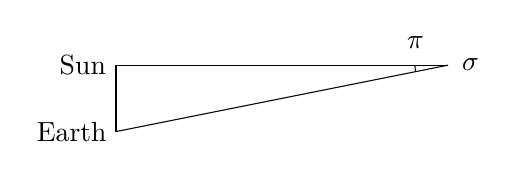
\begin{tikzpicture}[x=0.4pt, y=0.4pt, yscale=1, xscale=1]
\draw (0, 0) -- (300, 0);
\draw (0, 0) -- (0,-60);
\draw (0,-60) -- (300, 0);
\draw (270, 0) arc(180:190:30);
\draw (-30, 0) node {Sun};
\draw (-40,-60) node {Earth};
\draw (320, 0) node {$\sigma$};
\draw (270, 20) node {$\pi$};
\end{tikzpicture}
\captionsetup{justification=raggedright, singlelinecheck=false}
\caption{三角视差。}
\label{三角视差。}
\end{figure}

一条基线两端观测同一天体时,天体相对遥远背景天体发生位移,记位移前后天体方向单位矢量夹角为视差。视差显然与基线长度和天体距离有关。如三角视差采用日地距离作为基线,记日地距离平均值为一个天文单位 ($\unit{AU}$), $\qty{1}{AU}=\qty{1.496e8}{km}$, 记恒星到地球(或日心)距离为 $r$, 可用视差 $\pi$ 来表征距离:
\begin{equation}
\pi=\frac{\qty{1}{AU}}{r}.
\end{equation}
视差恰好为 $\ang{;; 1}$ 时,称恒星距离我们一秒差距 ($\unit{pc}$),
\begin{equation}
\qty{1}{pc}=\frac{\qty{1}{AU}}{\ang{;; 1}}=\frac{\qty{1}{AU}}{\dfrac{\ang{1;;}}{3600}\times\dfrac{\pi}{\ang{180;;}}}\approx\qty{206265}{AU}.
\end{equation}

\newpage
\section{站心坐标}
从天体到观测者的光线因通过地球大气层而产生弯曲,观测者测得的天体位置与没有大气时不同,方向差 $\rho=z-z_{\text{obs}}$ 称为大气折射。作了大气折射改正后得到的天体坐标为站心坐标。

\subsection{平面平行层大气}
我们从最简单的情况出发考虑大气折射近似公式,即认为大气层是 $N$ 个不同密度的平行平面均匀层组成。根据简单的折射定律可知
\begin{align}
n_{i}\sin{z_{i}}&=n_{i-1}\sin{z_{i-1}},\\
n_{0}\sin{z_{\text{obs}}}&=\sin{z}=\sin{\left(z_{\text{obs}}+\rho\right)}.
\end{align}
其中大气折射 $\rho$ 是小量,展开移项后得到
\begin{equation}
\rho=\left(n_{0}-1\right)\tan{z_{\text{obs}}}=R\tan{z_{\text{obs}}}.
\end{equation}
大气温度 $t=\qty{0}{\degreeCelsius}$, 大气压为 $H=\qty{760}{mmHg}$ 时,$R=n_{0}-1=\ang{;; 60.4}$.

天顶距不太大时也可使用下面两式描述大气折射:
\begin{align}
\rho&=\ang{;; 60.4}\frac{\dfrac{H}{\qty{760}{mmHg}}}{1+\dfrac{t}{\qty{273}{K}}}\tan{z_{\text{obs}}}.\\
\rho&=\ang{;; 21.3}\frac{\dfrac{H}{\unit{mmHg}}\left(1+\dfrac{0.00567}{\lambda^{2}}\right)}{\dfrac{t}{\unit{K}}+273}\tan{z_{\text{obs}}}.
\end{align}
其中 $\lambda$ 是以微米为单位的波长。

现在我们可以考虑大气折射引起的恒星位移。向点 $A$ 显然是天顶 $Z$, 记地理纬度 $\varphi$, 任一恒星赤道坐标观测值 $\sigma\left(\alpha,\delta{}\right)$, 时角为 $t$, 则天顶赤道坐标为 $\left(\alpha+t,\varphi\right)$. 改正是从 $z_{\text{obs}}$ 向 $z$ 移动,$k$ 取正值,因此 $\symup{d}\theta=\rho=z-z_{\text{obs}}=k\sin{\theta}=k\sin{z_{\text{obs}}}=R\tan{z_{\text{obs}}}$, 简单计算可知
\begin{align}
k&=R\sec{z_{\text{obs}}}.\\
\alpha'-\alpha&=k\sec{\delta}\cos{\varphi}\sin{\left(-t\right)},\\
\delta'-\delta&=k\left[\sin{\delta}\cos{\varphi}\cos{\left(-t\right)}-\cos{\delta}\sin{\varphi}\right].
\end{align}
接着在球面三角形 $\Delta{}PZ\sigma$ 中我们可以得到
\begin{equation}
\cos{z_{\text{obs}}}=\sin{\varphi}\sin{\delta}+\cos{\varphi}\cos{\delta}\cos{t},
\end{equation}
因此
\begin{align}
\alpha'-\alpha=-\frac{R\sec^{2}{\delta}\sin{t}}{\tan{\varphi}\tan{\delta}+\cos{t}},\\
\delta'-\delta=R\frac{\tan{\delta}\cos{t}-\tan{\varphi}}{\tan{\varphi}\tan{\delta}+\cos{t}}.
\end{align}

我们也可以考虑矢量方法,
\begin{align}
S&=\begin{pmatrix}
\cos{\delta}\cos{\alpha}\\
\cos{\delta}\sin{\alpha}\\
\sin{\delta}
\end{pmatrix},
S_{0}=\begin{pmatrix}
\cos{\varphi}\cos{\left(\alpha+t\right)}\\
\cos{\varphi}\sin{\left(\alpha+t\right)}\\
\sin{\varphi}
\end{pmatrix},\\
\vec{S}\cdot\vec{S}_{0}&=\cos{\delta}\cos{\varphi}\cos{t}+\sin{\delta}\sin{\varphi},\\
\begin{pmatrix}
-\sin{\alpha}\cos{\delta}\symup{d}\alpha-\cos{\alpha}\sin{\delta}\symup{d}\delta\\
\cos{\alpha}\cos{\delta}\symup{d}\alpha-\sin{\alpha}\sin{\delta}\symup{d}\delta\\
\cos{\delta}\symup{d}\delta
\end{pmatrix}&=k
\begin{pmatrix}
\cos{\delta}\cos{\alpha}\left(\cos{\delta}\cos{\varphi}\cos{t}+\sin{\delta}\sin{\varphi}\right)-\cos{\varphi}\cos{\left(a+t\right)}\\
\cos{\delta}\sin{\alpha}\left(\cos{\delta}\cos{\varphi}\cos{t}+\sin{\delta}\sin{\varphi}\right)-\cos{\varphi}\sin{\left(a+t\right)}\\
\sin{\delta}\left(\cos{\delta}\cos{\varphi}\cos{t}+\sin{\delta}\sin{\varphi}\right)-\sin{\varphi}
\end{pmatrix}.
\end{align}
整理得到
\begin{align}
\cos{\delta}\symup{d}\alpha&=-k\cos{\varphi}\sin{t},\\
\cos{\delta}\symup{d}\delta&=k\left(\sin{\delta}\cos{\delta}\cos{\varphi}\cos{t}-\cos^{2}{\delta}\sin{\varphi}\right),
\end{align}
最后可以得到与球面三角一致的结论。

\subsection{径向对称大气}
\begin{figure}[!htbp]
\centering
\begin{minipage}[t]{0.4\textwidth}
\tikzset{every picture/.style={line width=0.75pt}}
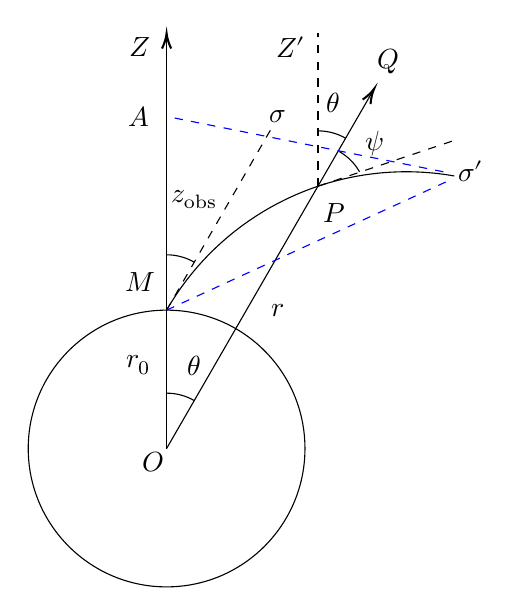
\begin{tikzpicture}[x=0.5pt, y=0.5pt, yscale=1, xscale=1]
\draw (100, 0) arc(0:360:100);
\draw (0, 0) -- (0, 300);
\draw [shift={(0, 300)}, rotate = -90] [color={rgb, 255: red, 0; green, 0; blue, 0 }  ][line width=0.75]    (10.93,-3.29) .. controls (6.95,-1.4) and (3.31,-0.3) .. (0, 0) .. controls (3.31, 0.3) and (6.95, 1.4) .. (10.93, 3.29);
\draw (0, 0) -- (150, 260);
\draw [shift={(150, 260)}, rotate = -120] [color={rgb, 255: red, 0; green, 0; blue, 0 }  ][line width=0.75]    (10.93,-3.29) .. controls (6.95,-1.4) and (3.31,-0.3) .. (0, 0) .. controls (3.31, 0.3) and (6.95, 1.4) .. (10.93, 3.29);
\draw (0, 100) arc(150:80:200);
\draw [dashed](0, 100) -- (75, 230);
\draw [dashed](109.44, 189.56) -- (109.44, 300);
\draw [dashed](109.44, 189.56) -- (209.44, 223.19);
\draw (0, 140) arc(90:60:40);
\draw (0, 40) arc(90:60:40);
\draw (109.44, 229.56) arc(90:60:40);
\draw (139.44, 200) arc(30:60:40);
\draw [dashed, blue](200, 200) -- (0, 240);
\draw [dashed, blue](0, 100) -- (207, 195);
%Text
\draw (-10,-10) node {$O$};
\draw (-20, 60) node {$r_{0}$};
\draw (80, 100) node {$r$};
\draw (-20, 120) node {$M$};
\draw (120, 170) node {$P$};
\draw (160, 280) node {$Q$};
\draw (-20, 290) node {$Z$};
\draw (90, 290) node {$Z'$};
\draw (80, 240) node {$\sigma$};
\draw (220, 200) node {$\sigma'$};
\draw (-20, 240) node {$A$};
\draw (20, 60) node {$\theta$};
\draw (20, 180) node {$z_{\text{obs}}$};
\draw (120, 250) node {$\theta$};
\draw (150, 220) node {$\psi$};
\end{tikzpicture}
\end{minipage}
\begin{minipage}[t]{0.4\textwidth}
\tikzset{every picture/.style={line width=0.75pt}}
\begin{tikzpicture}[x=0.5pt, y=0.5pt, yscale=0.8, xscale=0.8]
\draw (200, 200) arc(45:100:280);
\draw (300, 300) arc(45:100:420);
\draw (0, 0) -- (0, 480);
\draw (0, 0) -- (240, 415.7);
\draw (0, 281) -- (-100, 180);
\draw (0, 282) -- (210, 366);
\draw (210, 366) -- (350, 366);
\draw (220, 383) arc(60:0:20);
\draw (200, 349) arc(240:200:20);
\draw (0, 300) arc(90:30:20);
\draw (-20,-20) node {$O$};
\draw (20, 320) node {$\psi_{i}$};
\draw (270, 390) node {$\psi_{i+1}$};
\draw (180, 340) node {$\chi$};
\draw (200, 395) node {$P$};
\draw (-20, 300) node {$R$};
\draw (-40, 350) node {$n_{i}$};
\draw (-40, 450) node {$n_{i+1}$};
\draw (-20, 150) node {$r_{i}$};
\draw (140, 180) node {$r_{i+1}$};
\end{tikzpicture}
\end{minipage}
\captionsetup{justification=raggedright, singlelinecheck=false}
\caption{径向对称大气。}
\label{径向对称大气。}
\end{figure}

现在我们考虑径向对称大气。如图\ref{径向对称大气。}所示,$O$ 是地心,$M$ 是距离地心 $r_{0}$ 的观测者,$Z$ 是天顶方向,$P$ 是星光传播路径上的点,$\theta$ 是 $OP$ 与 $OZ$ 的夹角,$r$ 是地心距,因此 $P$ 可用极坐标 $\left(r,\theta\right)$ 表示。$\psi$ 表示每层大气星光入射角,$\chi$ 表示出射角,$n$ 是折射率,$z$ 是光线入射方向和天底方向的夹角,易得 $z=\psi+\theta$.

角 $\psi$ 实际描述了星光传播路径的变化,根据极坐标变化规律易得
\begin{equation}
\tan{\psi}=\frac{r\symup{d}\theta}{\symup{d}r}.
\end{equation}
因此
\begin{equation}
\symup{d}z=\symup{d}\psi+\symup{d}\theta=\symup{d}\psi+\frac{\tan{\psi}}{r}\symup{d}r.
\end{equation}

根据折射定律和几何关系可知
\begin{align}
n_{i+1}\sin{\psi_{i+1}}&=n_{i}\sin{\chi},\\
\frac{\sin{\chi}}{r_{i}}&=\frac{\sin{\psi_{i}}}{r_{i+1}},\\
r_{i+1}n_{i+1}\sin{\psi_{i+1}}&=r_{i}n_{i}\sin{\psi_{i}}=r_{0}n_{0}\sin{z_{\text{obs}}},\\
\tan{\psi}&=\frac{r_{0}n_{0}\sin{z_{\text{obs}}}}{\sqrt{r^{2}n^{2}-r_{0}^{2}n_{0}^{2}\sin^{2}{z_{\text{obs}}}}}.
\end{align}
微分 $rn\sin{\psi}=\symup{const}$ 得到
\begin{align}
&n\sin{\psi}\symup{d}r+r\sin{\psi}\symup{d}n+rn\cos{\psi}\symup{d}\psi=0,\notag\\
&\symup{d}\psi=-\frac{\tan{\psi}}{r}\symup{d}r-\frac{\tan{\psi}}{n}\symup{d}n,\notag\\
&\symup{d}z=-\frac{\tan{\psi}}{n}\symup{d}n.
\end{align}
积分就可得到大气折射引起的天顶距的变化,
\begin{equation}
\rho'=\int_{M}^{\sigma'}\symup{d}z=\int_{1}^{n_{0}}\frac{r_{0}n_{0}\sin{z_{\text{obs}}}}{n\sqrt{r^{2}n^{2}-r_{0}^{2}n_{0}^{2}\sin^{2}{z_{\text{obs}}}}}\symup{d}n.\label{2.2.8}
\end{equation}
之所以加角标是因为,$\rho'$ 还不是真正的大气折射。$\rho'$ 是 $M\sigma$ 和 $\sigma'$ 处光线切线 $A\sigma'$ 的夹角,$\rho$ 是 $M\sigma$ 和 $M\sigma'$ 的夹角,$\rho=\rho'-\angle{M\sigma'A}$. 现在我们先认为 $\rho=\rho'$.

现在的问题是我们不知道 $r$ 和 $n$ 的具体关系,只能作一些假设。首先令 $r=r_{0}+h$, 顺便记 $z_{\text{obs}}=z_{0}$, (\ref{2.2.8}) 式转化为
\begin{equation}
\rho=n_{0}\sin{z_{0}}\int_{1}^{n_{0}}\frac{\symup{d}n}{n\sqrt{\left(1+\dfrac{h}{r_{0}}^{2}\right)n^{2}-n_{0}^{2}\sin^{2}{z_{0}}}},
\end{equation}
天顶距不是非常大时,将上式展开成幂级数并保留零阶和一阶项,记作
\begin{align}
\rho&=\rho_{1}-\rho_{2}+O\left(\frac{h^{2}}{r_{0}^{2}}\right),\\
\rho_{1}&=n_{0}\sin{z_{0}}\int_{1}^{n_{0}}\frac{\symup{d}n}{n\sqrt{n^{2}-n_{0}^{2}\sin^{2}{z_{0}}}}=\arcsin\left(n_{0}\sin{z_{0}}\right)-z_{0},\\
\rho_{2}&=\frac{n_{0}\sin{z_{0}}}{r_{0}}\int_{1}^{n_{0}}\frac{hn\symup{d}n}{\left(n^{2}-n_{0}^{2}\sin^{2}{z_{0}}\right)^{\frac{3}{2}}},
\end{align}
如果将 $\rho_{1}$ 展开成 $n_{0}-1$ 的幂级数,仅保留到第二项可以得到
\begin{equation}
\rho_{1}=\left(n_{0}-1\right)\tan{z_{0}}+\frac{1}{2}\left(n_{0}-1\right)^{2}\tan^{3}{z_{0}},
\end{equation}
计算 $\rho_{2}$ 时,用大气密度代替大气折射率,
\begin{equation}
n=1+\left(n_{0}-1\right)\frac{\rho}{\rho_{0}},
\end{equation}
其中 $\rho_{0}$ 是地面处大气密度。保留到一阶项
\begin{align}
\rho_{2}&=\frac{\tan{z_{0}}\sec^{2}{z_{0}}}{r_{0}}\frac{n_{0}-1}{\rho_{0}}\int_{0}^{\rho_{0}}h\symup{d}\rho\notag\\
&=\left(n_{0}-1\right)\frac{H_{0}}{r_{0}}\tan{z_{0}}\sec^{2}{z_{0}},
\end{align}
其中标高
\begin{equation}
H_{0}=\frac{1}{\rho_{0}}\int_{0}^{\rho_{0}}h\symup{d}\rho=\frac{1}{\rho_{0}}\int_{0}^{\infty}\rho\symup{d}h.
\end{equation}

最终我们得到大气折射的形式
\begin{align}
\rho&=A\tan{z_{0}}+B\tan^{3}{z_{0}}+\cdots\\
A&=\left(n_{0}-1\right)\left(1-\frac{H_{0}}{r_{0}}\right),\\
B&=-\left(n_{0}-1\right)\left[\frac{H_{0}}{r_{0}}-\frac{1}{2}\left(n_{0}-1\right)\right].
\end{align}
实际情况往往取
\begin{equation}
\rho=\ang{;; 60.29}\tan{z_{0}}-\ang{;; 0.06688}\tan^{3}{z_{0}},
\end{equation}
可见天顶距较小时这与平面平行层大气结论接近。

我们还可根据 $\symup{d}\theta=\dfrac{\tan{\psi}}{r}\symup{d}r$ 计算光线传播路径上各点具体的极坐标:
\begin{align}
\theta&=r_{0}n_{0}\sin{z_{0}}\int_{r_{0}}^{r}\frac{\symup{d}r'}{r'\sqrt{{r'}^{2}n^{2}-r^{2}_{0}n_{0}^{2}\sin^{2}{z_{0}}}},\\
MA&=h_{0}=r_{0}\left[\frac{n_{0}\sin{z_{0}}}{\sin{\left(z_{0}+\rho\right)}}-1\right].
\end{align}
天顶距不大时,$h_{0}$ 很小,引起的视差变化 $\angle{M\sigma'A}$ 可以忽略不计,可认为 $\rho=\rho'$. 在观测地球人造卫星和地平附近的月球时此视差才重要。

\newpage
\section{地心坐标}
修正大气折射影响后,我们已经将观测坐标转换成了站心坐标。现在我们要考虑从观测站 $M$ 移动到地心 $O$ 所带来的影响。要考虑的因素有三个。首先,我们先前所考虑的地心其实不是真正的地心,所得到的天顶也其实是天文天顶。天文天顶是通过铅垂线确定的,但是地球并不是一个重力均匀体,并且地表各地离心力也不同,因此观测站和天文天顶的连线与观测站和真实地心的连线并不在一条直线上。我们需要修正这一点带来的影响。但是实际观测采用天文天顶很麻烦,我们可以采用测地天顶代替天文天顶(倒有点像平天极和真天极的关系)。为此需要定义重力位水准面,并取一个假想的与静止海水面相重合的重力位水准面作为大地水准面。大地水准面形状非常接近旋转椭球体,我们称其为参考椭球,并取参考椭球的法向作为测地天顶,随后便可将站心测地天顶值转换成站心地心天顶值。

其次,由于地球在自转且光速有限,运动中的观测者与静止观测者在同一瞬间观测到的天体方向是不同的,因此要考虑周日光行差改正,得到真正的站心地心天顶值。

最后,地心与地面上观测者看同一天体显然会有差别。随着地球自转,地心距引起的视差会发生变化,因此也被称为周日视差。修正后,站心地心天顶值将转换成地心地心天顶值。

\subsection{测地天顶}
参考椭球通常用半长轴 $a$ 和扁率 $f=\dfrac{a-b}{a}$ 来表示,IERS 规范中,$a=6378136.3,\dfrac{1}{f}=298.257$.
\begin{figure}[!htp]
\centering
\tikzset{every picture/.style={line width=0.75pt}}
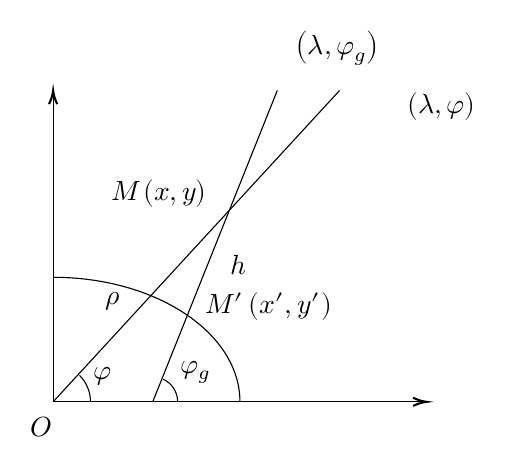
\begin{tikzpicture}[x=0.45pt, y=0.45pt, yscale=1, xscale=1]
\draw (0, 0) -- (0, 250);
\draw [shift={(0, 250)}, rotate=270][line width=0.75](10.93,-3.29) .. controls (6.95,-1.4) and (3.31,-0.3) .. (0, 0) .. controls (3.31, 0.3) and (6.95, 1.4) .. (10.93, 3.29); 
\draw (0, 0) -- (300, 0);
\draw [shift={(300, 0)}, rotate=180][line width=0.75](10.93,-3.29) .. controls (6.95,-1.4) and (3.31,-0.3) .. (0, 0) .. controls (3.31, 0.3) and (6.95, 1.4) .. (10.93, 3.29); 
%Text
\draw (0, 100) arc(90:0:150 and 100);
\draw (30, 0) arc(0:45:30);
\draw (100, 0) arc(0:65:20);
\draw (0, 0) -- (230, 250);
\draw (80, 0) -- (180, 250);
\draw (45, 180) node [anchor=north west][inner sep=0.75pt]   [align=left] {$M\left(x, y\right)$};
\draw (140, 120) node [anchor=north west][inner sep=0.75pt]   [align=left] {$h$};
\draw (-20,-10) node [anchor=north west][inner sep=0.75pt]   [align=left] {$O$};
\draw (40, 90) node [anchor=north west][inner sep=0.75pt]   [align=left] {$\rho$};
\draw (120, 90) node [anchor=north west][inner sep=0.75pt]   [align=left] {$M'\left(x', y'\right)$};
\draw (30, 30) node [anchor=north west][inner sep=0.75pt]   [align=left] {$\varphi$};
\draw (100, 35) node [anchor=north west][inner sep=0.75pt]   [align=left] {$\varphi_{g}$};
\draw (160, 300) node [anchor=north west][inner sep=0.75pt]   [align=left] {测地天顶 $\left(\lambda,\varphi_{g}\right)$};
\draw (250, 250) node [anchor=north west][inner sep=0.75pt]   [align=left] {地心天顶 $\left(\lambda,\varphi\right)$};
\end{tikzpicture}
\captionsetup{justification=raggedright, singlelinecheck=false}
\caption{测地天顶和地心天顶。}
\label{测地天顶和地心天顶。}
\end{figure}

因为近似标准椭球,因此测地天顶和地心天顶仅有地理纬度方向的差异,可以记二者坐标分别为 $\left(\lambda,\varphi_{g}\right)$ 和 $\left(\lambda,\varphi\right)$. 记站心位置为 $M\left(x, y\right)$, 地心距 $OM=\rho$, 对应大地水准面上的点为 $M'\left(x', y'\right)$, 海拔高度海拔高度 $MM'=h$. 具体几何关系可如图\ref{测地天顶和地心天顶。}所示。易知坐标关系满足
\begin{align}
\frac{x'^{2}}{a^{2}}&+\frac{y'^{2}}{a^{2}\left(1-f\right)^{2}}=1,\\
\tan{\varphi_{g}}&=-\dfrac{1}{\dfrac{\symup{d}y'}{\symup{d}x'}}=\frac{y'}{x'\left(1-f\right)^{2}},\\
x&=\rho\cos{\varphi}=x'+h\cos{\varphi_{g}},\\
y&=\rho\sin{\varphi}=y'+h\sin{\varphi_{g}}.
\end{align}
解得
\begin{align}
x'&=\frac{a\cos{\varphi_{g}}}{\sqrt{\cos^{2}{\varphi_{g}}+\left(1-f\right)^{2}\sin^{2}{\varphi_{g}}}}=ac\cos{\varphi_{g}},\\
y'&=ac\left(1-f\right)^{2}\sin{\varphi_{g}}=as\sin{\varphi_{g}},\\
\rho\cos{\varphi}&=a\left(c+\frac{h}{a}\right)\cos{\varphi_{g}},\\
\rho\sin{\varphi}&=a\left(s+\frac{h}{a}\right)\sin{\varphi_{g}}.
\end{align}
因此知道海拔 $h$ 和测地纬度 $\varphi_{g}$ 就可以计算地心距 $\rho$ 和地心纬度 $\varphi$ 了。

\subsection{周日光行差}
由于周日光行差修正很小,因此不考虑相对论效应,从经典图像出发。观测者 $M$ 有速度 $\vec{v}$, 等价于天体有速度 $-\vec{v}$, 观测者看到 $\sigma'$ 的时候,天体实际位置是 $\sigma$. 几何关系如图\ref{周日光行差。}所示。
\begin{figure}[!htp]
\centering
\tikzset{every picture/.style={line width=0.75pt}}
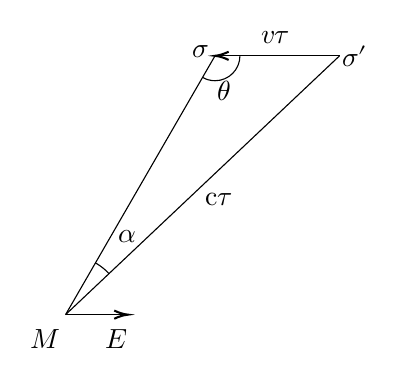
\begin{tikzpicture}[x=0.45pt, y=0.45pt, yscale=1, xscale=1]
\draw (0, 0) -- (120, 207.84);
\draw (24, 41.57) arc(60:43:48);
\draw (220, 207.84) -- (120, 207.84);
\draw (140, 207.84) arc(0:-120:20);
\draw (0, 0) -- (220, 207.84);
\draw [shift={(120, 207.84)}, rotate=0][line width=0.75](10.93,-3.29) .. controls (6.95,-1.4) and (3.31,-0.3) .. (0, 0) .. controls (3.31, 0.3) and (6.95, 1.4) .. (10.93, 3.29); 
\draw (0, 0) -- (50, 0);
\draw [shift={(50, 0)}, rotate=180][line width=0.75](10.93,-3.29) .. controls (6.95,-1.4) and (3.31,-0.3) .. (0, 0) .. controls (3.31, 0.3) and (6.95, 1.4) .. (10.93, 3.29); 
%Text
\draw (-30,-10) node [anchor=north west][inner sep=0.75pt]   [align=left] {$M$};
\draw (30,-10) node [anchor=north west][inner sep=0.75pt]   [align=left] {$E$};
\draw (220, 217.84) node [anchor=north west][inner sep=0.75pt]   [align=left] {$\sigma'$};
\draw (100, 217.84) node [anchor=north west][inner sep=0.75pt]   [align=left] {$\sigma$};
\draw (110, 100) node [anchor=north west][inner sep=0.75pt]   [align=left] {$\symup{c}\tau$};
\draw (155, 230) node [anchor=north west][inner sep=0.75pt]   [align=left] {$v\tau$};
\draw (40, 70) node [anchor=north west][inner sep=0.75pt]   [align=left] {$\alpha$};
\draw (120, 190) node [anchor=north west][inner sep=0.75pt]   [align=left] {$\theta$};
\end{tikzpicture}
\captionsetup{justification=raggedright, singlelinecheck=false}
\caption{周日光行差。}
\label{周日光行差。}
\end{figure}

记赤道地心距为 $a$, 赤道自转线速度 $v_{0}=\qty{0.4651}{km\cdot{}s^{-1}}$, 可知自转速度满足
\begin{equation}
v=\rho\cos{\varphi}\frac{v_{0}}{a}=\rho\omega\cos{\varphi}.
\end{equation}
地球自西向东旋转,可知恒星位移自东向西。但实际上我们考虑天体自 $\sigma$ 向 $\sigma'$ 的位移,取向点为东点 $E$, 此时 $k$ 是负值。$E$ 的赤道坐标为 $\left(S+\ang{90;;}, 0\right)$. 记 $E$ 与 $\sigma$ 夹角为 $\theta$, 恒星位移为 $\alpha$, 因为 $\alpha$ 是小量,由几何关系可知
\begin{align}
\sigma\sigma'&=\alpha\approx\sin{\alpha}=\frac{v}{\symup{c}}\sin{\theta},\\
k&=-\frac{v}{\symup{c}}=-\frac{\rho}{a}\frac{v_{0}}{\symup{c}}\cos{\varphi}=-\frac{\rho}{a}k'\cos{\varphi}.
\end{align}
其中周日光行差常数 $k'=\dfrac{v_{0}}{\symup{c}}=\ang{;; 0.320}$.

代入恒星位移公式得到
\begin{align}
\alpha'-\alpha&=\frac{\rho}{a}k'\cos{\varphi}\sec{\delta}\cos{t},\\
\delta'-\delta&=\frac{\rho}{a}k'\cos{\varphi}\sin{\delta}\sin{t}.
\end{align}
可见周日光行差引起的恒星位移会让天体在在天球上绘制出一个椭圆。根据此可确定天体的真实位置。注意,由于赤经方向是小圆,在天球上绘制的椭圆横轴是 $\left(\alpha'-\alpha\right)\cos{\delta}$.

\newpage
\subsection{周日视差}
\begin{figure}[!htbp]
\centering
\begin{minipage}[t]{0.45\textwidth}
\tikzset{every picture/.style={line width=0.75pt}}
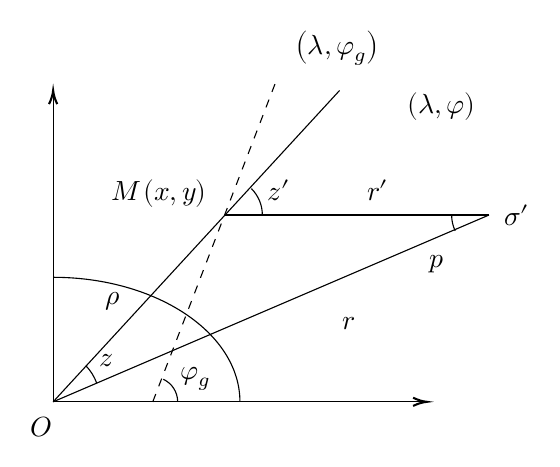
\begin{tikzpicture}[x=0.45pt, y=0.45pt, yscale=1, xscale=1]
\draw (0, 0) -- (0, 250);
\draw [shift={(0, 250)}, rotate=270][line width=0.75](10.93,-3.29) .. controls (6.95,-1.4) and (3.31,-0.3) .. (0, 0) .. controls (3.31, 0.3) and (6.95, 1.4) .. (10.93, 3.29); 
\draw (0, 0) -- (300, 0);
\draw [shift={(300, 0)}, rotate=180][line width=0.75](10.93,-3.29) .. controls (6.95,-1.4) and (3.31,-0.3) .. (0, 0) .. controls (3.31, 0.3) and (6.95, 1.4) .. (10.93, 3.29); 
%Text
\draw (0, 100) arc(90:0:150 and 100);
\draw (0, 0) -- (230, 250);
\draw (138, 150) -- (350, 150);
\draw (0, 0) -- (350, 150);
\draw (168, 150) arc(0:45:30);
\draw (35, 15) arc(20:44:40);
\draw (320, 150) arc(180:205:30);
\draw (45, 180) node [anchor=north west][inner sep=0.75pt]   [align=left] {$M\left(x, y\right)$};
\draw (360, 160) node [anchor=north west][inner sep=0.75pt]   [align=left] {$\sigma'$};
\draw (250, 180) node [anchor=north west][inner sep=0.75pt]   [align=left] {$r'$};
\draw (230, 70) node [anchor=north west][inner sep=0.75pt]   [align=left] {$r$};
\draw (-20,-10) node [anchor=north west][inner sep=0.75pt]   [align=left] {$O$};
\draw (40, 90) node [anchor=north west][inner sep=0.75pt]   [align=left] {$\rho$};
\draw (300, 120) node [anchor=north west][inner sep=0.75pt]   [align=left] {$p$};
\draw (170, 180) node [anchor=north west][inner sep=0.75pt]   [align=left] {$z'$};
\draw (35, 40) node [anchor=north west][inner sep=0.75pt]   [align=left] {$z$};
\draw (100, 0) arc(0:65:20);
\draw (100, 30) node [anchor=north west][inner sep=0.75pt]   [align=left] {$\varphi_{g}$};
\draw [dashed](80, 0) -- (180, 260);
\draw (160, 300) node [anchor=north west][inner sep=0.75pt]   [align=left] {测地天顶 $\left(\lambda,\varphi_{g}\right)$};
\draw (250, 250) node [anchor=north west][inner sep=0.75pt]   [align=left] {地心天顶 $\left(\lambda,\varphi\right)$};
\end{tikzpicture}
\end{minipage}
\begin{minipage}[t]{0.45\textwidth}
\tikzset{every picture/.style={line width=0.75pt}}
\begin{tikzpicture}[x=0.45pt, y=0.45pt, yscale=0.5, xscale=0.5]
% 天球
\draw (300, 0) arc(0:360:300);
% 三角形
\draw (240, 180) arc(-30:-63:390);
\draw (0, 300) arc(50:10:400);
%Text
\draw (20, 340) node {测地天顶 $Z'$};
\draw (300, 240) node {地心天顶 $Z$};
\draw (-260, 240) node {$P$};
\draw (80, 0) node {$\sigma'$};
\draw (80,-50) node {站心地心};
\draw (150, 50) node {$\sigma$};
\end{tikzpicture}
\end{minipage}
\captionsetup{justification=raggedright, singlelinecheck=false}
\caption{地心视差。}
\label{地心视差。}
\end{figure}

观测者从站心移动到地心时,观测得到的天体会向地心天顶移动,产生地心视差 $p=z'-z$. 图\ref{地心视差。}描述了这一过程,其中图\ref{地心视差。}左半图中天体 $\sigma'$ 并不位于纸面中,测地天顶 $Z'$ 地心天顶 $Z$ 和 $\sigma'$ 实际上组成一个球面三角形。给定 $O\sigma'=r, M\sigma'=r'$, 可见
\begin{equation}
\sin{p}=\frac{\rho}{r}\sin{z'}=\frac{\rho}{r'}\sin{z}.
\end{equation}

当地心距取 $a$, $z'=\ang{90;;}$ 时,地心视差最大,此时称其为地平视差
\begin{equation}
\sin{p_{0}}=\frac{a}{r}.
\end{equation}
如对太阳而言,$r=\qty{1}{AU},\sin{\pi_{\odot}}=\ang{;; 8.794148}$. 对遥远恒星可认为 $z'\approx z$.

现在我们来研究恒星位移。类似周日光行差,考虑站心地心观测值 $\sigma'$ 围绕地心地心观测值 $\sigma$ 而成的视差椭圆。向点为地心天顶 $Z\left(S,\varphi\right)$, 记 $\sigma\left(\alpha,\delta{}\right), S=\alpha+t$.
\begin{align}
k&=\frac{\rho}{r},\\
\alpha'-\alpha&=-k\sec{\delta}\cos{\varphi}\sin{t},\\
\delta'-\delta&=k\left(\sin{\delta}\cos{\varphi}\cos{t}-\cos{\delta}\sin{\varphi}\right).
\end{align}
天球上定义 $x=\left(\alpha'-\alpha\right)\cos{\delta}, y=\delta'-\delta$, 消去时角得到:
\begin{equation}
\frac{x^{2}}{\left(\cos{\varphi}\right)^{2}}+\frac{\left(y+\dfrac{\rho}{r}\cos{\delta}\sin{\varphi}\right)^{2}}{\left(\sin{\delta}\cos{\varphi}\right)^{2}}=\left(\frac{\rho}{r}\right)^{2}.
\end{equation}

$t=0$ 时,$\alpha'-\alpha=0,\delta'-\delta$ 最大,在椭圆最上方。

$t=\ang{90;;}$ 时,$\alpha'-\alpha$ 最小,$\delta'-\delta$ 取到“零点”,在椭圆左边。

因此从外面看天球,周日视差引起天体绕真实值逆时针旋转。对于观测者会发现恒星在作顺时针旋转。

当然我们也可以采用矢量方法分析。首先
\begin{equation}
\sin{p_{0}}=\frac{a}{r}\to{}r=a\csc{p_{0}}.
\end{equation}

天体的地心位置矢量为
\begin{equation}
\vec{r}=\begin{pmatrix}
a\csc{p_{0}}\cos{\delta}\cos{\alpha}\\
a\csc{p_{0}}\cos{\delta}\sin{\alpha}\\
a\csc{p_{0}}\sin{\delta}
\end{pmatrix}.
\end{equation}
观测者的地心位置矢量为
\begin{equation}
\vec{\rho}=\begin{pmatrix}
\rho\cos{\varphi}\cos{S}\\
\rho\cos{\varphi}\sin{S}\\
\rho\sin{\varphi}
\end{pmatrix}.
\end{equation}
天体的站心位置矢量为
\begin{equation}
\vec{r'}=\vec{r}-\vec{\rho}.
\end{equation}
如此可得
\begin{equation}
\begin{pmatrix}
r'\cos{\delta'}\cos{\alpha'}\\
r'\cos{\delta'}\sin{\alpha'}\\
r'\sin{\delta'}
\end{pmatrix}=
\begin{pmatrix}
a\csc{p_{0}}\cos{\delta}\cos{\alpha}-\rho\cos{\varphi}\cos{S}\\
a\csc{p_{0}}\cos{\delta}\sin{\alpha}-\rho\cos{\varphi}\sin{S}\\
a\csc{p_{0}}\sin{\delta}-\rho\sin{\varphi}
\end{pmatrix}.
\end{equation}
可见
\begin{equation}
\tan{\alpha'}=\frac{y'}{x'}=\frac{a\csc{p_{0}}\cos{\delta}\sin{\alpha}-\rho\cos{\varphi}\sin{S}}{a\csc{p_{0}}\cos{\delta}\cos{\alpha}-\rho\cos{\varphi}\cos{S}}=\frac{\sin{\alpha}-\dfrac{\rho}{a}\sin{p_{0}}\sec{\delta}\cos{\varphi}\sin{S}}{\cos{\alpha}-\dfrac{\rho}{a}\sin{p_{0}}\sec{\delta}\cos{\varphi}\cos{S}}.
\end{equation}
因此容易计算赤经方向的变化:
\begin{equation}
\tan{\left(\alpha'-\alpha\right)}=\frac{\tan{\alpha'}-\tan{\alpha}}{1+\tan{\alpha'}\tan{\alpha}}=\frac{-\dfrac{\rho}{a}\sin{p_{0}}\sec{\delta}\cos{\varphi}\sin{\left(S-\alpha\right)}}{1-\dfrac{\rho}{a}\sin{p_{0}}\sec{\delta}\cos{\varphi}\cos{\left(S-\alpha\right)}}=\frac{-\dfrac{\rho}{a}\sin{p_{0}}\sec{\delta}\cos{\varphi}\sin{t}}{1-\dfrac{\rho}{a}\sin{p_{0}}\sec{\delta}\cos{\varphi}\cos{t}}.
\end{equation}

对于赤纬,
\begin{equation}
\tan{\delta'}=\frac{z'}{\sqrt{x'^{2}+y'^{2}}}=\frac{a\csc{p_{0}}\sin{\delta}-\rho\sin{\varphi}}{\sqrt{a^{2}\csc^{2}{p_{0}}\cos^{2}{\delta}+\rho^{2}\cos^{2}{\varphi}-2a\csc{p_{0}}\cos{\delta}\rho\cos{\varphi}\cos{t}}}.
\end{equation}
可见用这个算 $\tan{\left(\delta'-\delta\right)}$ 有亿点复杂。采取另一种算法。

考虑
\begin{align}
r'\cos{\delta'}\cos{\alpha'}&=a\csc{p_{0}}\cos{\delta}\cos{\alpha}-\rho\cos{\varphi}\cos{S},\label{3.3.15}\\
r'\cos{\delta'}\sin{\alpha'}&=a\csc{p_{0}}\cos{\delta}\sin{\alpha}-\rho\cos{\varphi}\sin{S}.\label{3.3.16}
\end{align}
(\ref{3.3.15}) $\times\cos{\left(\dfrac{1}{2}\left(\alpha'+\alpha\right)\right)}+$ (\ref{3.3.16}) $\times\sin{\left(\dfrac{1}{2}\left(\alpha'+\alpha\right)\right)}$ 得到
\begin{align}
&r'\cos{\delta'}\cos{\left(\alpha'-\frac{1}{2}\left(\alpha'+\alpha\right)\right)}=a\csc{p_{0}}\cos{\delta}\cos{\left(\alpha-\frac{1}{2}\left(\alpha'+\alpha\right)\right)}-\rho\cos{\varphi}\cos{\left(S-\frac{1}{2}\left(\alpha'+\alpha\right)\right)},\\
&\left(r'\cos{\delta'}-a\csc{p_{0}}\cos{\delta}\right)\cos{\left(\frac{1}{2}\left(\alpha'-\alpha\right)\right)}=-\rho\cos{\varphi}\cos{\left(S-\frac{1}{2}\left(\alpha'+\alpha\right)\right)}.
\end{align}
引入辅助量满足
\begin{align}
\beta\sin{\gamma}&=\sin{\varphi},\\
\beta\cos{\gamma}&=\frac{\cos{\varphi}\cos{\left(S-\dfrac{1}{2}\left(\alpha'+\alpha\right)\right)}}{\cos{\left(\dfrac{1}{2}\left(\alpha'-\alpha\right)\right)}}=\frac{a\csc{p_{0}}\cos{\delta}-r'\cos{\delta'}}{\rho},
\end{align}
再考虑
\begin{equation}
r'\sin{\delta'}=a\csc{p_{0}}\sin{\delta}-\rho\sin{\varphi},
\end{equation}
结果是
\begin{align}
\sin{\delta'}&=\frac{a\csc{p_{0}}\sin{\delta}-\rho\sin{\varphi}}{r'},\\
\cos{\delta'}&=\frac{a\csc{p_{0}}\cos{\delta}-\rho\beta\cos{\gamma}}{r'},\\
\tan{\delta'}&=\frac{a\csc{p_{0}}\sin{\delta}-\rho\sin{\varphi}}{a\csc{p_{0}}\cos{\delta}-\rho\beta\cos{\gamma}}=\frac{a\csc{p_{0}}\sin{\delta}-\rho\beta\sin{\gamma}}{a\csc{p_{0}}\cos{\delta}-\rho\beta\cos{\gamma}},\\
\tan{\left(\delta'-\delta\right)}&=\frac{\tan{\delta'}-\tan{\delta}}{1+\tan{\delta'}\tan{\delta}}=\frac{-\dfrac{\rho}{a}\beta\sin{p_{0}}\sin{\left(\gamma-\delta\right)}}{1-\dfrac{\rho}{a}\beta\sin{p_{0}}\cos{\left(\gamma-\delta\right)}}.
\end{align}

\newpage
\section{日心或太阳系质心坐标(真位置)}
从地心坐标转换到日心坐标,我们要考虑地球公转引起的周年光行差和周年视差。由于行星到行星轨道焦点的距离并非定值,我们还将简单介绍一下如何用矢径 $r$, 真近点角 $f$, 平近点角 $M$, 偏近点角 $E$ 以及轨道半长轴 $a$, 轨道偏心率 $e$, 轨道对黄道倾角 $i$, 轨道升交点黄经 $\Omega$, 自轨道升交点逆时针计量的近日点角距离 $\omega$, 行星过近日点时刻 $\tau_{0}$, 轨道周期 $T$ 等 7 个 Campbell 轨道根数描述行星轨道。

\subsection{地球的绕日运动}
众所周知,行星轨道可以用开普勒三定律描述:
\begin{align}
r&=\frac{a\left(1-e^{2}\right)}{1+e\cos{f}},\\
h&=r^{2}\dot{f}=\frac{2\pi{}ab}{T}=\frac{2\pi}{T}a^{2}\sqrt{1-e^{2}},\\
\frac{a^{3}}{T^{2}}&=\frac{\symup{G}M}{4\pi^{2}}.
\end{align}
但是椭圆轨道的角速度并不恒定,要用均匀的时间系统描述,需要引入平近点角。为了计算平近点角,则要引入偏近点角。
\begin{figure}[!htp]
\centering
\tikzset{every picture/.style={line width=0.75pt}}
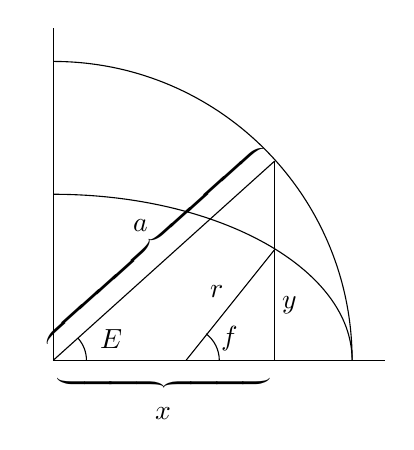
\begin{tikzpicture}[x=0.4pt, y=0.4pt, yscale=1, xscale=1]
\draw (0, 0) -- (0, 300);
\draw (0, 0) -- (300, 0);
\draw (0, 270) arc(90:0:270);
\draw (270, 0) arc(0:90:270 and 150);
\draw (0, 0) -- (200, 180);
\draw (120, 0) -- (200, 100);
\draw (200, 0) -- (200, 180);
\draw (30, 0) arc(0:42:30);
\draw (150, 0) arc(0:53:30);
%Text
\draw (40, 30) node [anchor=north west][inner sep=0.75pt]   [align=left] {$E$};
\draw (150, 33) node [anchor=north west][inner sep=0.75pt]   [align=left] {$f$};
\draw (205, 60) node [anchor=north west][inner sep=0.75pt]   [align=left] {$y$};
\draw (140, 70) node [anchor=north west][inner sep=0.75pt]   [align=left] {$r$};
\draw [rotate = 270] (20, 100) node {$\underbrace{\hspace{2.7cm}}$};
\node [rotate = 222] at (90, 105) {$\underbrace{\hspace{3.7cm}}$};
\draw (90,-40) node [anchor=north west][inner sep=0.75pt]   [align=left] {$x$};
\draw (70, 130) node [anchor=north west][inner sep=0.75pt]   [align=left] {$a$};
\end{tikzpicture}
\captionsetup{justification=raggedright, singlelinecheck=false}
\caption{真近点角 $f$ 与偏近点角 $E$.}
\label{真近点角与偏近点角。}
\end{figure}

如图\ref{真近点角与偏近点角。}所示,考虑椭圆轨道 $\dfrac{x^{2}}{a^{2}}+\dfrac{y^{2}}{b^{2}}=1$, 引入辅助圆 $\dfrac{x^{2}}{a^{2}}+\dfrac{y^{2}}{a^{2}}=1$. 根据相同横坐标时纵坐标的比例关系我们不难发现
\begin{align}
y&=r\sin{f}=a\sin{E}\sqrt{1-e^{2}},\label{4.1.4}\\
x&=ae+r\cos{f}=a\cos{E},\label{4.1.5}\\
r&=a\left(1-e\cos{E}\right).
\end{align}

偏近点角和平近点角的转换则用到了开普勒方程
\begin{equation}
M=E-e\sin{E}=\frac{2\pi}{T}\left(t-\tau_{0}\right).
\end{equation}

接着我们考虑椭圆轨道在天球上的投影。图\ref{轨道根数。}中 $X\text{\textendash}Y$ 平面是黄道面,$X$ 是春分点方向,$P$ 表示此时行星位置。很明显黄道坐标系中 $P$ 的坐标就是 $r$ 乘上其与三个坐标轴之间的夹角,即
\begin{equation}
\vec{r}=r\begin{pmatrix}
\cos{\overset{\frown}{PX}}\\
\cos{\overset{\frown}{PY}}\\
\cos{\overset{\frown}{PZ}}
\end{pmatrix}.
\end{equation}

\begin{figure}[!htp]
\centering
\tikzset{every picture/.style={line width=0.75pt}} 
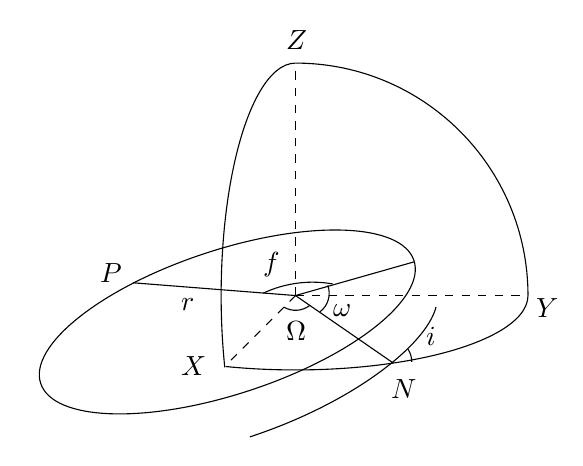
\begin{tikzpicture}[x=0.42pt, y=0.42pt, yscale=-1, xscale=1]
% 切平面坐标系 
\draw [dashed](300, 250) -- (500, 250);
\draw [dashed](300, 250) -- (300, 50);
\draw [dashed](300, 250) -- (240, 310);
% 天球
\draw (500, 250) arc(0:-90:200);
\draw (500, 250) arc(0:107.5:200 and 64);
\draw (300, 50) arc(270:162:64 and 200);
% 双星轨道
\draw (80.73, 325.53) .. controls (70.03, 293) and (133.25, 242.98) .. (221.94, 213.81) .. controls (310.62, 184.63) and (391.19, 187.35) .. (401.89, 219.87) .. controls (412.59, 252.4) and (349.37, 302.42) .. (260.69, 331.6) .. controls (172, 360.77) and (91.43, 358.06) .. (80.73, 325.53) -- cycle;
\draw (300, 250) -- (402, 221);% 近心点
\draw (300, 250) -- (384, 308);% 升交点
\draw (300, 250) -- (160, 239);% 行星位置
\draw (420.89, 259.87) .. controls (412.59, 292.4) and (349.37, 342.42) .. (260.69, 371.6);% 外环
%Text
\draw (200, 300) node [anchor=north west][inner sep=0.75pt]   [align=left] {$X$};
\draw (505, 250) node [anchor=north west][inner sep=0.75pt]   [align=left] {$Y$};
\draw (290, 20) node [anchor=north west][inner sep=0.75pt]   [align=left] {$Z$};
\draw (380, 320) node [anchor=north west][inner sep=0.75pt]   [align=left] {$N$};
\draw (400, 307) arc(0:-33:20);
\draw (410, 275) node [anchor=north west][inner sep=0.75pt]   [align=left] {$i$};
\draw (290, 260) arc(120:53:20);
\draw (290, 270) node [anchor=north west][inner sep=0.75pt]   [align=left] {$\Omega$};
\draw (321, 264) arc(53:-20:20);
\draw (330, 255) node [anchor=north west][inner sep=0.75pt]   [align=left] {$\omega$};
\draw (332, 240) arc(-80:-115:100);
\draw (270, 210) node [anchor=north west][inner sep=0.75pt]   [align=left] {$f$};
\draw (130, 220) node [anchor=north west][inner sep=0.75pt]   [align=left] {$P$};
\draw (200, 250) node [anchor=north west][inner sep=0.75pt]   [align=left] {$r$};
\end{tikzpicture}
\captionsetup{justification=raggedright, singlelinecheck=false}
\caption{轨道根数。}
\label{轨道根数。}
\end{figure}

我们可以用球面三角来计算夹角余弦,但不妨使用坐标轴旋转矩阵。记行星轨道平面坐标系中行星方向单位矢量为 $\vec{S}_{1}\left(f, 0\right)$, 黄道坐标系中行星方向单位矢量为 $\vec{S}\left(\lambda,\beta\right)$, 它们有如下关系:
\begin{align}
\vec{S}_{1}\left(f, 0\right)&=R_{z}\left(\omega\right)R_{x}\left(i\right)R_{z}\left(\Omega\right)\vec{S}\left(\lambda,\beta\right),\\
\vec{S}\left(\lambda,\beta\right)&=R_{z}\left(-\Omega\right)R_{x}\left(-i\right)R_{z}\left(-\omega\right)\vec{S}_{1}\left(f, 0\right)\notag\\
&=\begin{pmatrix}
\cos{\Omega} & -\sin{\Omega} & 0\\
\sin{\Omega} & \cos{\Omega} & 0\\
0 & 0 & 1
\end{pmatrix}
\begin{pmatrix}
1 & 0 & 0\\
0 & \cos{i} & -\sin{i}\\
0 & \sin{i} & \cos{i}
\end{pmatrix}
\begin{pmatrix}
\cos{\omega} & -\sin{\omega} & 0\\
\sin{\omega} & \cos{\omega} & 0\\
0 & 0 & 1
\end{pmatrix}
\begin{pmatrix}
\cos{f}\\
\sin{f}\\
0
\end{pmatrix}\notag\\
&=\begin{pmatrix}
\cos{\Omega}\cos{\left(\omega+f\right)}-\sin{\Omega}\cos{i}\sin{\left(\omega+f\right)}\\
\sin{\Omega}\cos{\left(\omega+f\right)}+\cos{\Omega}\cos{i}\sin{\left(\omega+f\right)}\\
\sin{i}\sin{\left(\omega+f\right)}
\end{pmatrix}.\label{4.1.10}
\end{align}

现在我们对行星轨道有了基本的了解,可以来研究地球的运动。很明显对于地球而言,$i=0$. 我们可以定义近日点黄经 $\pi=\Omega+\omega$, 利用 (\ref{4.1.4})(\ref{4.1.5})(\ref{4.1.10}) 式可以得到
\begin{equation}
\vec{r}=r\vec{S}\left(\lambda,\beta\right)=r\begin{pmatrix}
\cos{\left(f+\pi\right)}\\
\sin{\left(f+\pi\right)}\\
0
\end{pmatrix}=
\begin{pmatrix}
a\left(\cos{E}-e\right)\cos{\pi}-a\sqrt{1-e^{2}}\sin{E}\sin{\pi}\\
a\left(\cos{E}-e\right)\sin{\pi}+a\sqrt{1-e^{2}}\sin{E}\cos{\pi}\\
0
\end{pmatrix}.
\end{equation}

\begin{figure}[!htp]
\centering
\tikzset{every picture/.style={line width=0.75pt}}
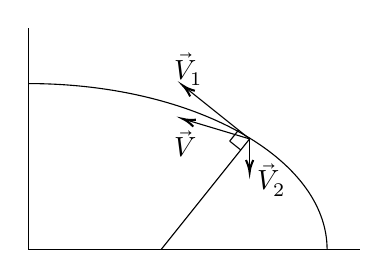
\begin{tikzpicture}[x=0.4pt, y=0.4pt, yscale=1, xscale=1]
\draw (0, 0) -- (0, 200);
\draw (0, 0) -- (300, 0);
\draw (270, 0) arc(0:90:270 and 150);
\draw (120, 0) -- (200, 100);
\draw (200, 100) -- (200, 70);
\draw (200, 100) -- (140, 148);
\draw (190, 108) -- (182, 98);
\draw (192, 90) -- (182, 98);
\draw (200, 100) -- (140, 118);
\draw [shift={(200, 70)}, rotate=90][line width=0.75](10.93,-3.29) .. controls (6.95,-1.4) and (3.31,-0.3) .. (0, 0) .. controls (3.31, 0.3) and (6.95, 1.4) .. (10.93, 3.29); 
\draw [shift={(140, 118)}, rotate=-20][line width=0.75](10.93,-3.29) .. controls (6.95,-1.4) and (3.31,-0.3) .. (0, 0) .. controls (3.31, 0.3) and (6.95, 1.4) .. (10.93, 3.29); 
\draw [shift={(140, 148)}, rotate=-40][line width=0.75](10.93,-3.29) .. controls (6.95,-1.4) and (3.31,-0.3) .. (0, 0) .. controls (3.31, 0.3) and (6.95, 1.4) .. (10.93, 3.29); 
%Text
\draw (130, 180) node [anchor=north west][inner sep=0.75pt]   [align=left] {$\vec{V}_{1}$};
\draw (205, 80) node [anchor=north west][inner sep=0.75pt]   [align=left] {$\vec{V}_{2}$};
\draw (130, 110) node [anchor=north west][inner sep=0.75pt]   [align=left] {$\vec{V}$};
\end{tikzpicture}
\captionsetup{justification=raggedright, singlelinecheck=false}
\caption{速度分解。}
\label{速度分解。}
\end{figure}

在计算周日光行差时我们考虑了地球的自转速度,那么在计算周年光行差时,我们也要确定地球的公转速度。如图\ref{速度分解。}所示,我们将切向速度 $\vec{V}$ 分解成垂直矢径方向的分量 $\vec{V}_{1}$ 和平行短轴方向的分量 $\vec{V}_{2}$, 根据几何关系可知
\begin{align}
\left\vert{}\vec{V}_{1}\right\vert{}&=r\frac{\symup{d}f}{\symup{d}t}-\cot{f}\frac{\symup{d}r}{\symup{d}t},\\
\left\vert{}\vec{V}_{2}\right\vert{}&=\csc{f}\frac{\symup{d}r}{\symup{d}t}.
\end{align}
根据开普勒第一和第二定律可以推出
\begin{align}
\frac{\symup{d}r}{\symup{d}t}&=\frac{he\sin{f}}{a\left(1-e^{2}\right)},\\
V_{1}&=\frac{h}{a\left(1-e^{2}\right)}=V_{0},\\
V_{2}&=eV_{0}.
\end{align}
考虑速度在黄道坐标系中的方向,
\begin{equation}
\vec{V}_{1}=V_{0}\begin{pmatrix}
-\sin{\left(f+\pi\right)}\\
\cos{\left(f+\pi\right)}\\
0
\end{pmatrix},
\vec{V}_{2}=eV_{0}\begin{pmatrix}
-\sin{\pi}\\
\cos{\pi}\\
0
\end{pmatrix},
\vec{V}=V_{0}\begin{pmatrix}
-\sin{\left(f+\pi\right)}-e\sin{\pi}\\
\cos{\left(f+\pi\right)}+e\cos{\pi}\\
0
\end{pmatrix}.
\end{equation}
实际过程还要考虑地球到地月系质心的修正以及日心到太阳系质心的修正。对于地月系质心,$a=\qty{0.999997}{AU}, e=0.016723, V_{0}=\qty{29.786}{km\cdot{}s^{-1}}$. 月球引起的位置改正与地月距离和质量有关,速度改正大小约 $\qty{12.5}{km\cdot{}s^{-1}}$; 日心和太阳系质心距离不到 $\qty{0.01}{AU}$, 太阳速度扰动主要由木星引起,大约对应 $\qty{10}{mas}$ 的光行差改正。

\subsection{周年光行差}
地球轨道近圆,取 $e=0$, 同时考虑 $\pi+f=-\lambda_{\odot}$, 因此速度在黄道坐标系中可写作
\begin{equation}
\vec{V}=V_{0}\begin{pmatrix}
\sin{\lambda_{\odot}}\\
-\cos{\lambda_{\odot}}\\
0
\end{pmatrix}.
\end{equation}
由于地球公转引起的光行差
\begin{equation}
\alpha=\frac{V_{0}}{\symup{c}}\sin{\theta}.
\end{equation}
其中 $\theta$ 是天体真方向和地球运动方向 $A$ 的夹角。很明显 $A$ 的黄道坐标是 $\left(\lambda_{\odot}-\ang{90;;}, 0\right)$, 利用黄赤坐标转换可得
\begin{equation}
\begin{pmatrix}
\cos{\delta_{A}}\cos{\alpha_{A}}\\
\cos{\delta_{A}}\sin{\alpha_{A}}\\
\sin{\delta_{A}}
\end{pmatrix}=\begin{pmatrix}
\sin{\lambda_{\odot}}\\
-\cos{\varepsilon}\cos{\lambda_{\odot}}\\
-\sin{\varepsilon}\cos{\lambda_{\odot}}
\end{pmatrix}.
\end{equation}
我们同样可以记光行差常数 $K=\dfrac{V_{0}}{\symup{c}}$, 可得恒星位移公式
\begin{align}
k&=-K,\\
\alpha'-\alpha&=k\sec{\delta}\cos{\delta_{A}}\sin{\left(\alpha-\alpha_{A}\right)}\notag\\
&=-K\sec{\delta}\cos{\delta_{A}}\left(\sin{\alpha}\cos{\alpha_{A}}-\cos{\alpha}\sin{\alpha_{A}}\right)\notag\\
&=-K\sec{\delta}\sin{\alpha}\sin{\lambda_{\odot}}-K\sec{\delta}\cos{\alpha}\cos{\varepsilon}\cos{\lambda_{\odot}},
\end{align}
\begin{align}
\delta'-\delta&=k\left[\sin{\delta}\cos{\delta_{A}}\cos{\left(\alpha-\alpha_{A}\right)}-\cos{\delta}\sin{\delta_{A}}\right]\notag\\
&=-K\cos{\lambda_{\odot}}\cos{\varepsilon}\left(\tan{\varepsilon}\cos{\delta}-\sin{\alpha}\sin{\delta}\right)-K\sin{\lambda_{\odot}}\cos{\alpha}\sin{\delta}.
\end{align}

如果化成更便于应用的形式,可以考虑赤道中地球速度矢量为
\begin{align}
\vec{V}_{E}&=\begin{pmatrix}
\dot{x}_{E}\\
\dot{y}_{E}\\
\dot{z}_{E}
\end{pmatrix}=V_{0}\begin{pmatrix}
\sin{\lambda_{\odot}}\\
-\cos{\lambda_{\odot}}\cos{\varepsilon}\\
-\cos{\lambda_{\odot}}\sin{\varepsilon}
\end{pmatrix}.\\
\alpha'-\alpha&=-\frac{1}{\symup{c}}\left(\dot{x}_{E}\sin{\alpha}\sec{\delta}-\dot{y}_{E}\cos{\alpha}\sec{\delta}\right),\\
\delta'-\delta&=-\frac{1}{\symup{c}}\left[\dot{x}_{E}\cos{\alpha}\sin{\delta}-\dot{y}_{E}\left(\tan{\varepsilon}\cos{\delta}-\sin{\alpha}\sin{\delta}\right)\right].
\end{align}
黄道坐标代入上式得到
\begin{align}
\lambda'-\lambda&=-K\sec{\beta}\cos{\left(\lambda-\lambda_{\odot}\right)},\\
\beta'-\beta&=K\sin{\beta}\sin{\left(\lambda-\lambda_{\odot}\right)}.
\end{align}

\subsection{周年视差}
有了周日视差的经验我们就不画示意图了。记日心为 $C$, 地球为 $E$, 日心系中恒星为 $\sigma$, 地心系中恒星为 $\sigma'$, $C\sigma=r, CE=R$, 周年视差为 $p$, 可见
\begin{equation}
\sin{p}=\frac{R}{r}\sin{\angle{\sigma{}EC}}.
\end{equation}
取 $R=a,\angle{\sigma{}EC}=\ang{90;;}$, 定义恒星的周年视差(简称恒星视差)
\begin{equation}
\sin{\pi}=\frac{a}{r}.
\end{equation}
在天球上考虑恒星位移时,延长 $EC$ 交天球于 $S, A$ 两点,从而记太阳方向为 $S,\angle{\sigma{}EC}=\overset{\frown}{\sigma'S}$, $A$ 的赤道坐标则是 $\left(\alpha_{\odot}-\ang{180;;},-\delta{}_{\odot}\right)$. 观测者从日心位移到地心时,天体向 $S$ 运动。
\begin{align}
\overset{\frown}{\sigma\sigma'}&=\frac{R}{r}\sin{\overset{\frown}{\sigma'S}}\approx\pi\sin{\overset{\frown}{\sigma{}S}}=\pi\sin{\overset{\frown}{\sigma{}A}},\\
\alpha'-\alpha&=\pi\cos{\delta_{\odot}}\sin{\left(\alpha_{\odot}-\alpha\right)}\sec{\delta},\\
\delta'-\delta&=\pi\left[\cos{\delta}\sin{\delta_{\odot}}-\sin{\delta}\cos{\delta_{\odot}}\cos{\left(\alpha_{\odot}-\alpha\right)}\right].
\end{align}
如果考虑黄道坐标系,取 $A\left(\lambda_{\odot}+\ang{180;;}, 0\right)$
\begin{align}
\lambda'-\lambda&=\pi\sec{\beta}\sin{\left(\lambda_{\odot}-\lambda\right)},\\
\beta'-\beta&=-\pi\sin{\beta}\cos{\left(\lambda_{\odot}-\lambda\right)}.
\end{align}
因此恒星在天球上描绘出一个视差椭圆,关于黄道对称,长半轴 $\pi$ 平行于黄道
\begin{equation}
\frac{x^{2}}{\pi^{2}}+\frac{y^{2}}{\pi^{2}\sin^{2}{\beta}}=1.
\end{equation}
恒星位移公式是矢量方法的一阶近似,若要寻求更精确的做法,可仿照周日视差部分。

\section{岁差、章动、极移}
上一章节我们得到了观测历元真赤道坐标系的日心坐标,经过章动改正后可改正到观测历元平赤道坐标系的日心坐标,再经过岁差改正和自行改正(岁差和自行改正一起做是因为岁差对自行也有影响)可以得到星表历元的平赤道坐标系位置。我们将在这一章节研究岁差和章动的影响,在下一章节研究自行的影响。

由于地球赤道有隆起部分,日月引力作用产生力矩作用,从天球外看,北天极在绕北黄极作顺时针运动,轨迹大致上可看作一条波浪线,该运动可被分解为平天极 $P_{0}$ 绕北黄极 $K$ 的小圆运动(日月岁差)和真天极 $P$ 绕平天极的运动(章动)。日月岁差周期约 25800 年,春分点黄经每世纪西移约 $\ang{;; 5029}$. 章动则十分复杂,如果忽略掉短周期的微小运动,可认为章动部分是顺时针(从天球外看)的椭圆运动,周期约 18.6 年。我们可以根据平天极和真天极各自定义平赤道、平春分点、真赤道、真春分点。每一时刻天体的平赤道坐标都在发生变化。

此外,由于行星对地球公转轨道的摄动,北黄极本身也会发生运动,这种影响叫行星岁差。这种影响比日月岁差小得多,春分点位置每世纪改变 $\ang{;; 12}$, 黄赤交角每世纪改变 $\ang{;; 47}$.

岁差和章动改变黄极和天极位置,极移与它们不同。由于地球瞬时自转轴和它的惯量椭球最短惯量主轴不重合,地球的自转轴会在没有外力的情况下发生变化,这被称作极移。当然,考虑到许许多多其他因素(比如大气层复杂的气象过程),地球自转轴的移动情况更加复杂。极移会导致观测台站的地理位置发生变化,从而改变观测台站的天顶。

\subsection{总岁差}
首先考虑日月岁差对赤道坐标的影响。由于春分点 $\gamma$ 是 $\overset{\frown}{KP_{0}}$ 所在大圆的极,因此在黄道坐标系中,春分点和平天极的黄经始终相差 $\ang{90;;}$. 设 $P_{0}$ 黄经角速度为 $\psi$, 可见春分点在黄道上运动速度也是 $\psi$. 因此我们也将日月岁差称作黄道岁差,$\psi$ 是黄经日月岁差速率。很明显 $\psi$ 可以在赤道坐标系中分解,赤经方向 $\psi\cos{\varepsilon}$, 赤纬方向 $\psi\sin{\varepsilon}$.(当然,实际坐标变化速率没有这么简单。)后者其实有着物理意义。由于春分点 $\gamma$ 是 $\overset{\frown}{KP_{0}}$ 所在大圆的极,所以当 $P_{0}$ 绕 $K$ 作小圆运动时,$P_{0}$ 速度方向实际上正指向 $\gamma$. 由于 $\overset{\frown}{KP_{0}}=\varepsilon$, 所以小圆半径是 $\sin{\varepsilon},\psi\sin{\varepsilon}$ 正好是北天极运动的线速度除以天球半径(单位一)的结果。

日月岁差对黄道坐标的影响可以表示为
\begin{equation}
\symup{d}\lambda=\psi\symup{d}t,\symup{d}\beta=0,\symup{d}\varepsilon=0,
\end{equation}
利用坐标系旋转可以得到日月岁差对赤道坐标的影响
\begin{align}
\symup{d}\alpha&=\psi\left(\cos{\varepsilon}+\sin{\varepsilon}\sin{\alpha}\tan{\delta}\right)\symup{d}t,\\
\symup{d}\delta&=\psi\sin{\varepsilon}\cos{\alpha}\symup{d}t.
\end{align}

考虑行星岁差时,我们则认为 $P_{0}$ 固定不动,$K$ 绕着 $P_{0}$ 逆时针(从天球外看)运动,因此春分点在赤道上东移(因此也被称作赤道岁差),并且有非常简单的关系:
\begin{equation}
\symup{d}\alpha=-\chi\symup{d}t,\symup{d}\delta=0.
\end{equation}
但计算行星岁差对黄道坐标的影响却并非如此容易,因为行星岁差影响了黄赤交角。首先考虑坐标变换
\begin{align}
\cos{\beta}\cos{\lambda}&=\cos{\delta}\cos{\alpha},\label{5.1.5}\\
\sin{\beta}&=\cos{\varepsilon}\sin{\delta}-\sin{\varepsilon}\cos{\delta}\sin{\alpha},\label{5.1.6}\\
\cos{\beta}\sin{\lambda}&=\sin{\delta}\sin{\varepsilon}+\cos{\delta}\cos{\varepsilon}\sin{\alpha},\label{5.1.7}\\
\cos{\delta}\sin{\alpha}&=-\sin{\beta}\sin{\varepsilon}+\cos{\beta}\cos{\varepsilon}\sin{\lambda},\label{5.1.8}
\end{align}
微分 (\ref{5.1.5})(\ref{5.1.6}) 式得到
\begin{align}
\cos{\beta}\sin{\lambda}\symup{d}\lambda+\sin{\beta}\cos{\lambda}\symup{d}\beta&=\cos{\delta}\sin{\alpha}\symup{d}\alpha=-\chi\cos{\delta}\sin{\alpha}\symup{d}t,\\
\cos{\beta}\symup{d}\beta&=-\sin{\delta}\sin{\varepsilon}\symup{d}\varepsilon-\cos{\delta}\left(\cos{\varepsilon}\sin{\alpha}\symup{d}\varepsilon+\sin{\varepsilon}\cos{\alpha}\symup{d}\alpha\right).
\end{align}
将 (\ref{5.1.7})(\ref{5.1.8}) 式代入其中,整理得到
\begin{align}
\symup{d}\lambda&=\left(\tan{\beta}\sin{\varepsilon}\sin{\lambda}-\cos{\varepsilon}\right)\chi\symup{d}t+\tan{\beta}\cos{\lambda}\symup{d}\varepsilon,\\
\symup{d}\beta&=\sin{\varepsilon}\cos{\lambda}\chi\symup{d}t-\sin{\lambda}\symup{d}\varepsilon.
\end{align}

现在我们需要知道黄赤交角具体的变化 $\symup{d}\varepsilon$. 将黄道的运动拆分为倾角和升交点位置的变化。首先,随着黄极的变化,变化前后的黄道交于 $N'N$ 两点,便可以用以 $N'$ 为顶点的夹角变化速率 $\pi$ 描述倾角的变化。记 $N$ 的黄经为 $\Pi$, 则 $N'$ 与变化前春分点 $\gamma$ 间的夹角为 $\ang{180;;}-\Pi$. 我们便可以利用球面三角 $\Delta{}N'\gamma\gamma'$ 来研究行星岁差。注意,$N'\gamma$ 位于变化前黄道,$N'\gamma'$ 位于变化后黄道,$\gamma\gamma'$ 位于平赤道,这些关系有助于我们确定边角关系。
\begin{figure}[!htp]
\centering
\tikzset{every picture/.style={line width=0.75pt}}
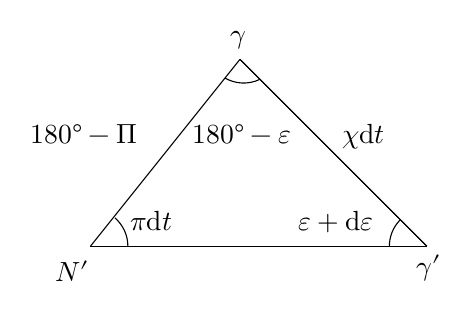
\begin{tikzpicture}[x=0.45pt, y=0.45pt, yscale=1, xscale=1]
\draw (0, 0) -- (120, 150);
\draw (30, 0) arc(0:49:30);
\draw (240, 0) arc(180:135:30);
\draw (0, 0) -- (270, 0);
\draw (120, 150) -- (270, 0);
\draw (120, 150) -- (270, 0);
\draw (108, 135) arc(-120:-65:30);
%Text
\draw (110, 175) node [anchor=north west][inner sep=0.75pt]   [align=left] {$\gamma$};
\draw (-30,-10) node [anchor=north west][inner sep=0.75pt]   [align=left] {$N'$};
\draw (260,-5) node [anchor=north west][inner sep=0.75pt]   [align=left] {$\gamma'$};
\draw (-50, 100) node [anchor=north west][inner sep=0.75pt]   [align=left] {$\ang{180;;}-\Pi$};
\draw (80, 100) node [anchor=north west][inner sep=0.75pt]   [align=left] {$\ang{180;;}-\varepsilon$};
\draw (200, 100) node [anchor=north west][inner sep=0.75pt]   [align=left] {$\chi\symup{d}t$};
\draw (165, 30) node [anchor=north west][inner sep=0.75pt]   [align=left] {$\varepsilon+\symup{d}\varepsilon$};
\draw (30, 30) node [anchor=north west][inner sep=0.75pt]   [align=left] {$\pi\symup{d}t$};
\end{tikzpicture}
\captionsetup{justification=raggedright, singlelinecheck=false}
\caption{球面三角 $\Delta{}N'\gamma\gamma'$.}
\label{球面三角 111.}
\end{figure}

运用正弦定理和四元素公式可得
\begin{align}
\cos{\left(\chi\symup{d}t\right)}\cos{\left(\ang{180;;}-\varepsilon\right)}&=\sin{\left(\chi\symup{d}t\right)}\cot{\left(\ang{180;;}-\pi\right)}-\sin{\left(\ang{180;;}-\varepsilon\right)}\cot{\left(\varepsilon+\symup{d}\varepsilon\right)},\\
\sin{\left(\chi\symup{d}t\right)}\sin{\left(\varepsilon+\symup{d}\varepsilon\right)}&=\sin{\Pi}\sin{\left(\pi\symup{d}t\right)},\\
\chi&=\pi\sin{\Pi}\csc{\varepsilon},\\
\symup{d}\varepsilon&=\pi\cos{\Pi}\symup{d}t.
\end{align}
代入之前的结果得到行星岁差对黄道坐标的影响
\begin{align}
\symup{d}\lambda&=-\chi\cos{\varepsilon}\symup{d}t+\pi\tan{\beta}\cos{\left(\Pi-\lambda\right)}\symup{d}t,\\
\symup{d}\beta&=\pi\sin{\left(\Pi-\lambda\right)}\symup{d}t,
\end{align}

总岁差就是上述两种要素的总和。此外我们还可以定义黄经总岁差速率 $p=\psi-\chi\cos{\varepsilon}$, 赤经总岁差速率 $m=\psi\cos{\varepsilon}-\chi$ 以及赤纬岁差速率 $n=\psi\sin{\varepsilon}$, 从而有
\begin{align}
\symup{d}\alpha&=\left(m+n\sin{\alpha}\tan{\delta}\right)\symup{d}t,\symup{d}\delta=n\cos{\alpha}\symup{d}t,\\
\symup{d}\lambda&=p\symup{d}t+\pi\tan{\beta}\cos{\left(\Pi-\lambda\right)}\symup{d}t,\symup{d}\beta=\pi\sin{\left(\Pi-\lambda\right)}\symup{d}t.
\end{align}

总岁差还会影响天体的轨道根数。为方便起见,我们考虑轨道对变化前黄道升交点为 $L$, 对变化后黄道升交点为 $L'$ 以及 $N$ 点组成的球面三角形。三条边分别是行星轨道和变化前后两条黄道。因为近日点“绝对位置”没有发生变化,因此升交点间的距离就是近心点幅角的变化量。
\begin{figure}[!htp]
\centering
\tikzset{every picture/.style={line width=0.75pt}}
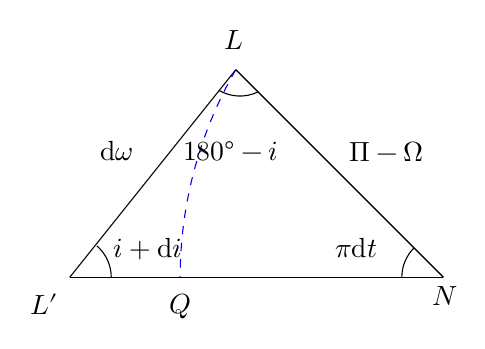
\begin{tikzpicture}[x=0.5pt, y=0.5pt, yscale=1, xscale=1]
\draw (0, 0) -- (120, 150);
\draw (30, 0) arc(0:49:30);
\draw (240, 0) arc(180:135:30);
\draw [dashed, blue](120, 150) arc(150:180:300);
\draw (0, 0) -- (270, 0);
\draw (120, 150) -- (270, 0);
\draw (120, 150) -- (270, 0);
\draw (108, 135) arc(-120:-65:30);
%Text
\draw (110, 180) node [anchor=north west][inner sep=0.75pt]   [align=left] {$L$};
\draw (-30,-10) node [anchor=north west][inner sep=0.75pt]   [align=left] {$L'$};
\draw (260,-5) node [anchor=north west][inner sep=0.75pt]   [align=left] {$N$};
\draw (70,-10) node [anchor=north west][inner sep=0.75pt]   [align=left] {$Q$};
\draw (20, 100) node [anchor=north west][inner sep=0.75pt]   [align=left] {$\symup{d}\omega$};
\draw (80, 100) node [anchor=north west][inner sep=0.75pt]   [align=left] {$\ang{180;;}-i$};
\draw (200, 100) node [anchor=north west][inner sep=0.75pt]   [align=left] {$\Pi-\Omega$};
\draw (190, 30) node [anchor=north west][inner sep=0.75pt]   [align=left] {$\pi\symup{d}t$};
\draw (30, 30) node [anchor=north west][inner sep=0.75pt]   [align=left] {$i+\symup{d}i$};
\end{tikzpicture}
\captionsetup{justification=raggedright, singlelinecheck=false}
\caption{球面三角 $LL'N$.}
\label{球面三角 222.}
\end{figure}

如图\ref{球面三角 222.}所示,过 $L$ 点以 $N$ 为极作小圆交 $L'N$ 为 $Q$, $L'Q$ 反映了黄道岁差和 $\Omega$ 的变化量,可以记 $\overset{\frown}{L'Q}=p\symup{d}t-\symup{d}\Omega$. 将 $\Delta{}LL'Q$ 看作平面直角三角形,并利用 $\Delta{}LL'N$ 的四元素公式得到
\begin{align}
\symup{d}\omega&=\pi\csc{i}\sin{\left(\Pi-\Omega\right)}\symup{d}t,\\
\symup{d}i&=-\pi\cos{\left(\Pi-\Omega\right)}\symup{d}t,\\
\symup{d}\Omega&=p\symup{d}t-\pi\cot{i}\sin{\left(\Pi-\Omega\right)}\symup{d}t.
\end{align}

\subsection{岁差量表达式、极图、岁差计算}
历元即时刻,计算某一起算历元(如 1950.0) 到另一目标历元(如 2000.0) 的岁差量时,需要用到三个历元,分别是:标准历元(基本历元)$t_{0}$, 起算历元(固定历元)$t_{s}$ 和目标历元(观测历元)$t_{D}$. 定义历元间隔世纪数:
\begin{equation}
T=\frac{t_{s}-t_{0}}{100}, t=\frac{t_{D}-t_{s}}{100},
\end{equation}
特别地,若取起算历元为标准历元 J2000.0, 此时 $T=0$.

我们将岁差量和岁差速率表示为时间间隔的幂级数:
\begin{align}
X_{A}&=\left(x_{1}+x_{2}T+x_{3}T^{2}\right)t+\left(x_{1}'+x_{2}'T\right)t^{2}+x_{1}''t^{3},\\
x&=\frac{\symup{d}X_{A}}{\symup{d}t}=x_{1}+x_{2}T+x_{3}T^{2}.
\end{align}
岁差量有十余种,都可以写成类似的形式,如 $t_{s}, t_{D}$ 黄道间夹角 $\pi_{A}$, 赤道间夹角 $\theta_{A}$; $t_{D}$ 黄道对 $t_{s}$ 黄道升交点 $N$ 在 $t_{s}$ 黄道的黄经 $\Pi_{A}$, $t_{D}$ 赤道对 $t_{s}$ 赤道升交点 $M$ 在 $t_{s}$ 赤道的赤经 $\ang{90;;}-\zeta_{A}$, $M$ 在 $t_{D}$ 赤道的赤经 $\ang{90;;}+z_{A}$. 根据定义我们不难发现在 $t_{s}$ 黄道坐标系中,变化后北黄极 $K_{D}$ 黄道坐标是 $\left(\Pi_{A}-\ang{90;;},\ang{90;;}-\pi_{A}\right)$, 以及赤经岁差 $m_{A}=\zeta_{A}+z_{A}$, 赤纬岁差 $n_{A}=\theta_{A}$. 具体而言我们可以用极图来描述各岁差量,如图\ref{极图。}所示。

\begin{figure}[!htp]
\centering
\tikzset{every picture/.style={line width=0.75pt}}
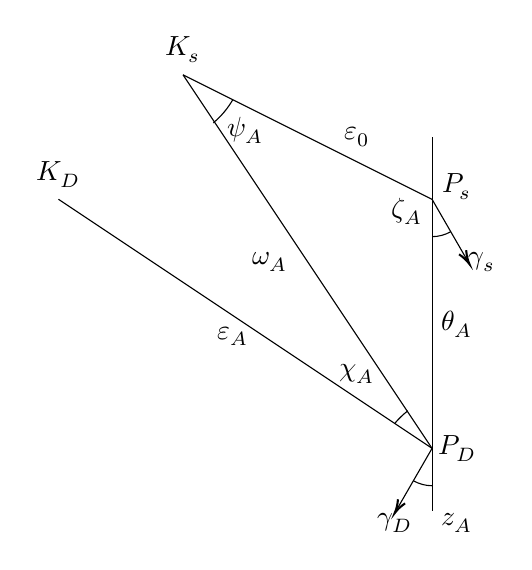
\begin{tikzpicture}[x=0.45pt, y=0.45pt, yscale=1, xscale=1]
\draw (0, 100) -- (300,-100);
\draw (100, 200) -- (300,-100);
\draw (300,-150) -- (300, 150);
\draw (100, 200) -- (300, 100);
\draw (300, 100) -- (330, 48);
\draw (300, 70) arc(-90:-60:30);
\draw (300,-100) -- (270,-152);
\draw (300,-130) arc(-90:-120:30);
\draw (140, 180) arc(-30:-50:70);
\draw (270,-80) arc(140:128:70);
\draw (100, 220) node {$K_{s}$};
\draw (0, 120) node {$K_{D}$};
\draw (320, 110) node {$P_{s}$};
\draw (340, 50) node {$\gamma_{s}$};
\draw (320,-100) node {$P_{D}$};
\draw (270,-160) node {$\gamma_{D}$};
\draw (320,-160) node {$z_{A}$};
\draw (320, 0) node {$\theta_{A}$};
\draw (280, 90) node {$\zeta_{A}$};
\draw (150, 155) node {$\psi_{A}$};
\draw (240,-40) node {$\chi_{A}$};
\draw (170, 50) node {$\omega_{A}$};
\draw (140,-10) node {$\varepsilon_{A}$};
\draw (240, 150) node {$\varepsilon_{0}$};
\draw [shift={(330, 48)}, rotate=120][line width=0.75](10.93,-3.29) .. controls (6.95,-1.4) and (3.31,-0.3) .. (0, 0) .. controls (3.31, 0.3) and (6.95, 1.4) .. (10.93, 3.29); 
\draw [shift={(270,-152)}, rotate=60][line width=0.75](10.93,-3.29) .. controls (6.95,-1.4) and (3.31,-0.3) .. (0, 0) .. controls (3.31, 0.3) and (6.95, 1.4) .. (10.93, 3.29); 
\end{tikzpicture}
\captionsetup{justification=raggedright, singlelinecheck=false}
\caption{极图。}
\label{极图。}
\end{figure}

图\ref{极图。}作图其实有误差,实际上 $\angle{K_{s}P_{s}\gamma_{s}}=\angle{K_{D}P_{D}\gamma_{D}}=\ang{90;;}$. 我们可以将 $P_{D}$ 向 $\gamma_{D}$ 运动的速度 $n=\psi\sin{\varepsilon_{A}}$ 投影到平行于和垂直于 $P_{s}P_{D}$, 以及平行于和垂直于 $K_{s}P_{D}$ 的方向。可以得到
\begin{align}
\symup{d}\theta_{A}&=n\symup{d}t\cos{z_{A}},\\
\sin{\theta_{A}}\symup{d}\zeta_{A}&=n\symup{d}t\sin{z_{A}},\\
\symup{d}\omega_{A}&=n\symup{d}t\sin{\chi_{A}},\\
\sin{\omega_{A}}\symup{d}\psi_{A}&=n\symup{d}t\cos{\chi_{A}}.
\end{align}

现在我们用岁差矩阵计算岁差。
\begin{figure}[!htp]
\centering
\tikzset{every picture/.style={line width=0.75pt}}
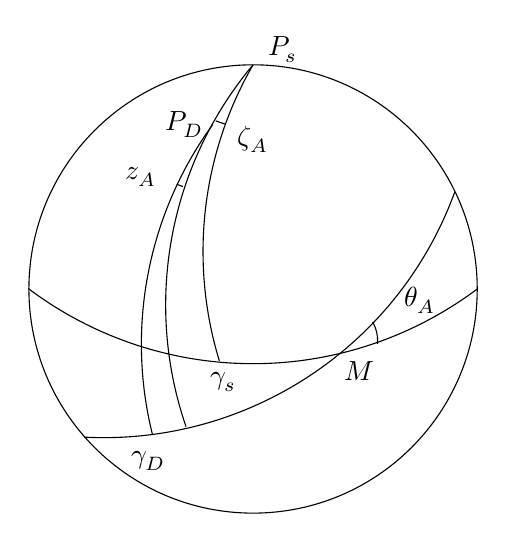
\begin{tikzpicture}[x=0.45pt, y=0.45pt, yscale=0.6, xscale=0.6]
% 天球
\draw (300, 0) arc(0:360:300);
% 基本圈
\draw (0,-100) arc(270:307:500);
\draw (0,-100) arc(270:233:500);
\draw (270, 130) arc(-20:-93:500);
\draw (160,-44) arc(30:-5:50);
\draw (223,-15) node {$\theta_{A}$};
\draw (0, 300) arc(140:199:500);
\draw (0, 300) arc(150:197:500);
\draw (-54, 220) arc(144:194:500);
\draw (-50, 225) arc(250:251.5:500);
\draw (-102, 140) arc(250:251:500);
%Text
\draw (-140,-230) node {$\gamma_{D}$};
\draw (-40,-125) node {$\gamma_{s}$};
\draw (-92, 220) node {$P_{D}$};
\draw (140,-110) node {$M$};
\draw (40, 320) node {$P_{s}$};
\draw (0, 200) node {$\zeta_{A}$};
\draw (-150, 150) node {$z_{A}$};
\end{tikzpicture}
\captionsetup{justification=raggedright, singlelinecheck=false}
\caption{岁差对赤道坐标的影响。}
\label{岁差对赤道坐标的影响。}
\end{figure}

如图\ref{岁差对赤道坐标的影响。}所示,赤道坐标系自 $t_{s}$ 向 $t_{D}$ 变换满足:绕 $z$ 轴转动 $\ang{90;;}-\zeta_{A}$, 绕 $x$ 轴转动 $\theta_{A}$, 绕 $z$ 轴转动 $-\ang{90;;}-z_{A},\vec{S}_{D}=R_{Z}\left(-\ang{90;;}-z_{A}\right)R_{X}\left(\theta_{A}\right)R_{Z}\left(\ang{90;;}-\zeta_{A}\right)\vec{S}_{s}=R_{Z}\left(-z_{A}\right)R_{Y}\left(\theta_{A}\right)R_{Z}\left(-\zeta_{A}\right)\vec{S}_{s}$.

我们可以定义岁差矩阵和它的一阶近似
\begin{equation}
P=R_{Z}\left(-z_{A}\right)R_{Y}\left(\theta_{A}\right)R_{Z}\left(-\zeta_{A}\right)\approx\begin{pmatrix}
1 & -\zeta_{A}-z_{A} & -\theta_{A}\\
\zeta_{A}+z_{A} & 1 & 0\\
\theta_{A} & 0 & 1
\end{pmatrix}.
\end{equation}
我们可以利用赤经岁差 $m_{A}=\left(\psi\cos{\varepsilon}-\chi\right)t$ 和赤纬岁差 $n_{A}=\psi\sin{\varepsilon}t$ 来表示岁差矩阵
\begin{equation}
P=\begin{pmatrix}
1 & -m_{A} & -n_{A}\\
m_{A} & 1 & 0\\
n_{A} & 0 & 1
\end{pmatrix}.
\end{equation}

当然也可以不用矩阵法而是考虑 $\Delta{}P_{s}P_{D}\sigma$ 组成的三角形,总之会得到如下结果
\begin{align}
\cos{\delta_{D}}\cos{\left(\alpha_{D}-z_{A}\right)}&=-\cos{\theta_{A}}\cos{\delta_{s}}\cos{\left(\alpha_{s}+\zeta_{A}\right)}+\sin{\theta_{A}}\sin{\delta_{s}},\\
\cos{\delta_{D}}\sin{\left(\alpha_{D}-z_{A}\right)}&=\cos{\delta_{s}}\sin{\left(\alpha_{s}+\zeta_{A}\right)},\\
\sin{\delta_{D}}&=\sin{\theta_{A}}\cos{\delta_{s}}\cos{\left(\alpha_{s}+\zeta_{A}\right)}+\cos{\theta_{A}}\sin{\delta_{s}}.
\end{align}

\subsection{章动}
我们提到过,章动可分为黄经章动和交角章动。前者是北天极黄经的变化,因此春分点在黄道上移动 $\Delta{}\psi$, 后者是北天极黄纬 $\Delta{}\beta$ 的变化,根据极与大圆性质,黄赤交角变化 $\Delta{}\varepsilon=\Delta{}\beta$. 章动影响天体的赤经、赤纬、黄经,但不影响天体的黄纬。

考虑黄赤坐标变换(其实我们在计算行星岁差时在 (\ref{5.1.5})\text{\textendash}(\ref{5.1.8}) 式做过类似的事情)以及球面三角形 $KP\sigma$,
\begin{align}
\cos{\alpha}\cos{\delta}&=\cos{\lambda}\cos{\beta},\\
\sin{\delta}&=\cos{\varepsilon}\sin{\beta}+\sin{\varepsilon}\cos{\beta}\sin{\lambda},\\
\cos{\beta}\sin{\lambda}&=\sin{\delta}\sin{\varepsilon}+\cos{\delta}\sin{\alpha}\cos{\varepsilon},\\
\symup{d}\alpha&=\left(\cos{\varepsilon}+\sin{\varepsilon}\sin{\alpha}\tan{\delta}\right)\Delta\psi-\cos{\alpha}\tan{\delta}\Delta\varepsilon,\\
\symup{d}\delta&=\sin{\varepsilon}\cos{\alpha}\Delta\psi+\sin{\alpha}\Delta\varepsilon.
\end{align}
上述依旧是一阶近似,严格公式要用矢量方法。仿照岁差矩阵我们可以列出章动矩阵以及它的一阶近似
\begin{equation}
N=R_{X}\left(-\varepsilon-\Delta\varepsilon\right)R_{Z}\left(-\Delta\psi\right)R_{X}\left(\varepsilon\right)\approx\begin{pmatrix}
1 & -\Delta{}\mu & -\Delta{}\nu\\
\Delta{}\mu & 1 & -\Delta{}\varepsilon\\
\Delta{}\nu & \Delta{}\varepsilon & 1
\end{pmatrix}.
\end{equation}
其中 $\Delta{}\mu=\Delta{}\psi\cos{\varepsilon},\Delta{}\nu=\Delta{}\psi\sin{\varepsilon}$.

\subsection{极移}
观测表明地极在 $\ang{;; 0.8}\times\ang{;; 0.8}$ 的范围内运动,我们可用平面代替这一范围内的球面,取 $x$ 正方向为平极(这里的平极指的是地极一定时间范围内平均指向)指向格林尼治子午线方向,$y$ 正方向为平极指向格林尼治子午线以西 $\ang{90;;}$ 方向。定义地理坐标 $\left(\lambda,\varphi\right)$, 极距 $\rho$ 和位置角 $\theta$, 利用
\begin{equation}
\begin{pmatrix}
\cos{\varphi}\cos{\lambda}\\
\cos{\varphi}\sin{\lambda}\\
\sin{\varphi}
\end{pmatrix}=R_{X}\left(y\right)R_{Y}\left(x\right)
\begin{pmatrix}
\cos{\varphi_{0}}\cos{\lambda_{0}}\\
\cos{\varphi_{0}}\sin{\lambda_{0}}\\
\sin{\varphi_{0}}
\end{pmatrix}
\end{equation}
和近似容易得到
\begin{align}
\begin{pmatrix}
\cos{\varphi}\cos{\lambda}\\
\cos{\varphi}\sin{\lambda}\\
\sin{\varphi}
\end{pmatrix}&=
\begin{pmatrix}
\cos{\varphi_{0}}\cos{\lambda_{0}}-x\sin{\varphi_{0}}\\
\cos{\varphi_{0}}\sin{\lambda_{0}}+y\sin{\varphi_{0}}\\
x\cos{\varphi_{0}}\cos{\lambda_{0}}-y\cos{\varphi_{0}}\sin{\lambda_{0}}+\sin{\varphi_{0}}
\end{pmatrix}.\\
\lambda-\lambda_{0}&=\left(x\sin{\lambda_{0}}+y\cos{\lambda_{0}}\right)\tan{\varphi_{0}},\\
\varphi-\varphi_{0}&=x\cos{\lambda_{0}}-y\sin{\lambda_{0}}.
\end{align}

\newpage
\section{恒星的运动}
如果恒星全部静止不动,经过章动和岁差改正后我们已经得到了星表历元太阳系质心平赤道坐标。但实际上恒星相对太阳有速度,这会引起坐标位移,且这种位移随观测历元和定向历元发生改变。为此我们需要研究恒星的运动。确定恒星的自行后,对观测历元太阳系质心真赤道坐标系坐标进行章动改正后可得观测历元太阳系质心平赤道坐标系坐标,再进行岁差和自行改正可得星表历元太阳系质心平赤道坐标系坐标。

记恒星速度为 $\vec{V}$, 恒星方向单位矢量 $\vec{S}$, 可见视向速度 $\vec{V}_{r}$ 和切向速度 $\vec{V}_{\text{T}}$ 满足
\begin{align}
\vec{V}_{r}&=\left(\vec{V}\cdot\vec{S}\right)\vec{S}, V_{r}=V\sin{\theta}=\frac{\symup{d}r}{\symup{d}t},\\
\vec{V}_{\text{T}}&=\left(\vec{S}\times\vec{V}\right)\times\vec{S}, V_{\text{T}}=V\cos{\theta}=r\frac{\symup{d}\theta}{\symup{d}t}.
\end{align}
过太阳作恒星速度矢量的垂线,天体方向单位矢量与垂线的夹角为 $\theta$, 具体如图\ref{恒星速度。}所示。
\begin{figure}[!htp]
\centering
\tikzset{every picture/.style={line width=0.75pt}}
\begin{tikzpicture}[x=0.5pt, y=0.5pt, yscale=1, xscale=1]
\draw (0, 0) -- (120, 120);
\draw [dashed](0, 0) -- (0, 120);
\draw [dashed](-30, 120) -- (120, 120);
\draw (0, 30) arc(90:45:30);
\draw (120, 120) -- (150, 120);
\draw [shift={(150, 120)}, rotate=180][line width=0.75](10.93,-3.29) .. controls (6.95,-1.4) and (3.31,-0.3) .. (0, 0) .. controls (3.31, 0.3) and (6.95, 1.4) .. (10.93, 3.29); 
\draw (15, 60) node [anchor=north west][inner sep=0.75pt]   [align=left] {$\theta$};
\draw (60, 60) node [anchor=north west][inner sep=0.75pt]   [align=left] {$r$};
\draw (150, 120) node [anchor=north west][inner sep=0.75pt]   [align=left] {$\vec{V}$};
\draw (-20, 0) node [anchor=north west][inner sep=0.75pt]   [align=left] {$O$};
\end{tikzpicture}
\captionsetup{justification=raggedright, singlelinecheck=false}
\caption{恒星速度。}
\label{恒星速度。}
\end{figure}

\subsection{恒星的视向速度}
恒星的视向速度可通过光谱的多普勒频移测定,长期来看变化很小,主要考虑日心到站心的修正。记恒星相对站心、地心、日心视向速度分别为 $V_{r}'', V_{r}', V_{r}$. 设恒星方向的单位矢量为 $\vec{S}$, 则地心和日心视向速度为
\begin{align}
V_{r}'&=V_{r}''+\vec{v}'\cdot\vec{S},\\
V_{r}&=V_{r}'+\vec{v}\cdot\vec{S}.
\end{align}
其中 $\vec{v}'$ 是观测者相对地心的速度,$\vec{v}$ 是地心相对日心的速度。前者与周日光行差相联系,始终指向东点,一定精度下可以取 $v'=v_{0}\cos{\varphi}$, 其中 $v_{0}=\qty{0.465}{km\cdot{}s^{-1}}$, $\varphi$ 是站心地理纬度。记恒星赤纬为 $\delta{}$, 时角为 $t$,
\begin{equation}
\vec{v}'\cdot\vec{S}=-v'\cos{\delta}\sin{t}.
\end{equation}
后者与周年光行差相联系,可以分解成切向速度 $\vec{v}_{1}$ 和平行地球短轴速度 $\vec{v}_{2}$. 记地球近日点黄经为 $\pi$, 黄道坐标系中
\begin{align}
\vec{v}_{1}&=V_{0}\begin{pmatrix}
\sin{\lambda_{\odot}}\\
-\cos{\lambda_{\odot}}\\
0
\end{pmatrix},
\vec{v}_{2}=eV_{0}\begin{pmatrix}
-\sin{\pi}\\
\cos{\pi}\\
0
\end{pmatrix}.\\
\vec{v}\cdot\vec{S}&=V_{0}\left[\cos{\beta}\sin{\left(\lambda_{\odot}-\lambda\right)}+e\cos{\beta}\sin{\left(\lambda-\pi\right)}\right].
\end{align}

\subsection{恒星的自行}
恒星的切向速度通过根据恒星自行和恒星距离确定。定义恒星自行
\begin{equation}
\mu=\frac{\symup{d}\theta}{\symup{d}t}.
\end{equation}
恒星距离 $r$ 可用恒星视差 $\pi$ 表示,
\begin{equation}
r=\frac{\qty{1}{AU}}{\pi},
\end{equation}
切向速度为
\begin{equation}
V_{\text{T}}=\qty{1}{AU}\cdot\frac{\mu}{\pi},
\end{equation}
如果取 $\pi$ 单位为角秒,$\mu$ 单位为角秒每年,$V_{\text{T}}$ 单位为 $\unit{km\cdot{}s^{-1}}$, 并令字母仅代表数值,则
\begin{equation}
V_{\text{T}}=4.74\frac{\mu}{\pi}.
\end{equation}

时间单位用年表示的恒星自行被称为恒星的周年自行,也称总自行。它沿赤经和赤纬方向分解为赤经周年自行 $\mu_{\alpha}$ 和赤纬周年自行 $\mu_{\delta}$. 考虑天极 $P$, 位移前的恒星 $\sigma$, 位移后的恒星 $\sigma'$, 记 $\angle{P\sigma\sigma'}$ 为位置角 $\varphi$, 自行是个小量,可认为赤经方向运动了 $\mu\symup{d}t\sin{\varphi}$, 赤纬方向运动了 $\mu\symup{d}t\cos{\varphi}$. 由于赤经方向的变化位于小圆上,而小圆的半径是 $\cos{\delta}$ 而非大圆的单位一,因此赤经变化和赤经方向实际的角度变化有偏差,
\begin{align}
\mu_{\alpha}&=\frac{\symup{d}\alpha}{\symup{d}t}=\mu\sin{\varphi}\sec{\delta},\label{6.2.5}\\
\mu_{\delta}&=\frac{\symup{d}\delta}{\symup{d}t}=\mu\cos{\varphi}.\label{6.2.6}
\end{align}

研究银河系恒星运动时常选择银道坐标系,自行可沿银经银纬方向分解:
\begin{align}
\mu_{l}\cos{b}&=\mu_{\alpha}\cos{\delta}\cos{\psi}+\mu_{\delta}\sin{\psi}\\
\mu_{b}&=\mu_{\delta}\cos{\psi}-\mu_{\alpha}\cos{\delta}\sin{\psi}.
\end{align}
其中 $\psi$ 是北银极和北天极的连线在恒星处所张的球面角,被称为银道星位角,从银经圈逆时针方向计量到赤经圈,根据四元素公式可推出
\begin{equation}
\cot{\psi}=\cot{i}\cos{\delta}\sec{\left(\alpha-\alpha_{N}\right)}+\sin{\delta}\tan{\left(\alpha-\alpha_{N}\right)}.
\end{equation}
空间速度可拆分成视向速度、切向速度的银经分量和银纬分量:
\begin{equation}
\vec{V}=\begin{pmatrix}
V_{x}\\
V_{y}\\
V_{z}
\end{pmatrix}=\begin{pmatrix}
V_{r}\cos{l}\cos{b}-V_{l}\sin{l}-V_{b}\cos{l}\sin{b}\\
V_{r}\sin{l}\cos{b}+V_{l}\cos{l}-V_{b}\sin{l}\sin{b}\\
V_{r}\sin{b}+V_{b}\cos{b}
\end{pmatrix}.
\end{equation}

严格来讲,自行是恒星相对天球惯性参考系而产生的位置变化。通常地说,恒星位置矢量由一个位置历元 $t$ 和一个定向历元 $T$ 定向的参考系所决定。位置历元的变换按自行来作,定向历元的变换(参考系的变换)按岁差来作。

恒星位置随位置历元 $t$ 的变换可以表示为泰勒级数
\begin{align}
\alpha&=\alpha_{0}+\frac{\symup{d}\alpha}{\symup{d}t}\left(t-t_{0}\right)+\frac{1}{2}\frac{\symup{d}^{2}\alpha}{\symup{d}t^{2}}\left(t-t_{0}\right)^{2}+\cdots\\
\delta&=\delta_{0}+\frac{\symup{d}\delta}{\symup{d}t}\left(t-t_{0}\right)+\frac{1}{2}\frac{\symup{d}^{2}\delta}{\symup{d}t^{2}}\left(t-t_{0}\right)^{2}+\cdots
\end{align}
很明显恒星坐标一阶导数就是自行,二阶导数则是自行的固有变化。微分 (\ref{6.2.5})(\ref{6.2.6}) 式得到
\begin{align}
\frac{\symup{d}\mu_{\alpha}}{\symup{d}t}&=\sin{\varphi}\sec{\delta}\frac{\symup{d}\mu}{\symup{d}t}+\mu\cos{\varphi}\sec{\delta}\frac{\symup{d}\varphi}{\symup{d}t}+\mu\sin{\varphi}\frac{\sin{\delta}}{\cos^{2}{\delta}}\frac{\symup{d}\delta}{\symup{d}t},\label{6.2.13}\\
\frac{\symup{d}\mu_{\delta}}{\symup{d}t}&=\cos{\varphi}\frac{\symup{d}\mu}{\symup{d}t}-\mu\sin{\varphi}\frac{\symup{d}\varphi}{\symup{d}t}.\label{6.2.14}
\end{align}
球面三角 $\Delta{}P\sigma\sigma'$ 是个小三角形,运用正弦公式发现
\begin{equation}
\sin{\varphi}\cos{\delta}\approx\sin{\varphi'}\cos{\delta'}=\symup{const},
\end{equation}
因此
\begin{align}
&\cos{\varphi}\cos{\delta}\frac{\symup{d}\varphi}{\symup{d}t}-\sin{\varphi}\sin{\delta}\frac{\symup{d}\delta}{\symup{d}t}=0,\notag\\
&\frac{\symup{d}\varphi}{\symup{d}t}=\tan{\varphi}\tan{\delta}\frac{\symup{d}\delta}{\symup{d}t}=\mu\sin{\varphi}\tan{\delta}=\mu_{\alpha}\sin{\delta}.
\end{align}

再根据自行定义 ($V$ 可被视作常数)
\begin{equation}
V\cos{\theta}=r\frac{\symup{d}\theta}{\symup{d}t},
\end{equation}
有
\begin{align}
-V\sin{\theta}\frac{\symup{d}\theta}{\symup{d}t}&=\frac{\symup{d}r}{\symup{d}t}\frac{\symup{d}\theta}{\symup{d}t}+r\frac{\symup{d}\mu}{\symup{d}t},\notag\\
r\frac{\symup{d}\mu}{\symup{d}t}&=-2V\sin{\theta}\mu,\notag\\
\frac{\symup{d}\mu}{\symup{d}t}&=-\frac{2V_{r}\mu\pi}{\qty{1}{AU}}.
\end{align}
因此 (\ref{6.2.13})(\ref{6.2.14}) 式可写作
\begin{align}
\frac{\symup{d}\mu_{\alpha}}{\symup{d}t}&=2\mu_{\alpha}\mu_{\delta}\tan{\delta}-\frac{2V_{r}\mu_{\alpha}\pi}{\qty{1}{AU}},\\
\frac{\symup{d}\mu_{\delta}}{\symup{d}t}&=-\mu_{\alpha}^{2}\sin{\delta}\cos{\delta}-\frac{2V_{r}\mu_{\delta}\pi}{\qty{1}{AU}},
\end{align}
取 $\mu_{\alpha}$ 单位为 $\unit{s\cdot yr^{-1}}$, $\mu_{\delta}$ 单位为 $\unit{arcsec\cdot yr^{-1}}$, $\pi$ 单位为 $^{\prime\prime}$, $V_{r}$ 单位为 $\unit{km\cdot{}s^{-1}}$, 则数值上写作
\begin{align}
\frac{\symup{d}\mu_{\alpha}}{\symup{d}t}&=2\mu_{\alpha}\mu_{\delta}\tan{\delta}-\frac{2V_{r}\mu_{\alpha}\pi}{1.496\times10^{8}\left(\unit{km}\right)}\times\frac{3.156\times10^{7}\left(\unit{s}\right)}{1\left(\unit{yr}\right)}\\
&=2\mu_{\alpha}\mu_{\delta}\tan{\delta}-0.422V_{r}\mu_{\alpha}\pi\quad\left(\unit{s\cdot arcsec\cdot yr^{-2}}\right),\\
\frac{\symup{d}\mu_{\delta}}{\symup{d}t}&=-225\mu_{\alpha}^{2}\sin{\delta}\cos{\delta}-0.422V_{r}\mu_{\delta}\pi\quad\left(\unit{arcsec^{2}\cdot yr^{-2}}\right).\label{6.2.23}
\end{align}
请注意角秒与时秒的区别,如此 (\ref{6.2.23}) 式第一项才会因 $\mu_{\alpha}^{2}$ 单位转换出现 $15^{2}$ 这个因子。

进行这种位置和自行的变换需要知道 $t_{0}$ 时刻恒星的位置、自行、距离和视向速度。但目前只有少数恒星的视向速度是已知的,距离测定很多情况下反而依赖观测结果。二者都未知时通常假设它们等于零。

恒星位置相对于参考系的变化也可以用旋转矩阵表示,有
\begin{align}
\vec{S}\left(\alpha,\delta\right)&=M\vec{S}\left(\alpha_{0},\delta_{0}\right),\\
M&=R_{Z}\left(-\alpha_{0}\right)R_{Y}\left(\delta_{0}-\ang{90;;}\right)R_{Z}\left(\varphi_{0}\right)R_{Y}\left(\mu_{0}\tau\right)R_{Z}\left(-\varphi_{0}\right)R_{Y}\left(\ang{90;;}-\delta_{0}\right)R_{Z}\left(\alpha_{0}\right).\\
\tau&=t-t_{0}.
\end{align}

现在考虑定向历元 $T$ 对自行的影响。参考系变换导致恒星自行在赤经圈和赤纬圈上的分量不断重新分配:
\begin{align}
\frac{\symup{d}\mu_{\alpha}}{\symup{d}T}&=\sin{\varphi}\sec{\delta}\frac{\symup{d}\mu}{\symup{d}T}+\mu\cos{\varphi}\sec{\delta}\frac{\symup{d}\varphi}{\symup{d}T}+\mu\sin{\varphi}\frac{\sin{\delta}}{\cos^{2}{\delta}}\frac{\symup{d}\delta}{\symup{d}T},\\
\frac{\symup{d}\mu_{\delta}}{\symup{d}T}&=\cos{\varphi}\frac{\symup{d}\mu}{\symup{d}T}-\mu\sin{\varphi}\frac{\symup{d}\varphi}{\symup{d}T}.
\end{align}
因为行星岁差不影响赤纬和方向位置角,我们仅考虑日月岁差。日月岁差不改变自行大小,$\dfrac{\symup{d}\mu}{\symup{d}T}=0$, 只引起赤纬方向的变化 $\dfrac{\symup{d}\delta{}}{\symup{d}t}=n\cos{\alpha}=\psi\sin{\varepsilon}\symup{d}t$ 和位置方向角 $\varphi$ 的变化。因此我们只需再得知 $\dfrac{\symup{d}\varphi}{\symup{d}t}$ 就可了解定向历元对自行的影响。

\begin{figure}[!htp]
\centering
\tikzset{every picture/.style={line width=0.75pt}}
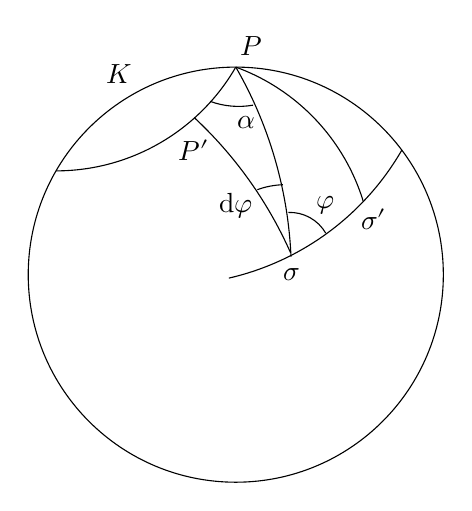
\begin{tikzpicture}[x=0.5pt, y=0.5pt, yscale=0.5, xscale=0.5]
% 天球
\draw (300, 0) arc(0:360:300);
% 三角形
\draw (0, 300) arc(-30:-90:300);
\draw (240, 180) arc(-30:-77:390);
\draw (0, 300) arc(70:17:300);
\draw (0, 300) arc(30:2.5:600);
\draw (-60, 227) arc(47:24:600);
\draw (130, 60) arc(30:92:60);
\draw (25, 245) arc(-80:-110:120);
\draw (68, 130) arc(92:110:120);
%Text
\draw (20, 330) node {$P$};
\draw (-60, 180) node {$P'$};
\draw (-170, 290) node {$K$};
\draw (80, 0) node {$\sigma$};
\draw (200, 80) node {$\sigma'$};
\draw (130, 100) node {$\varphi$};
\draw (0, 100) node {$\symup{d}\varphi$};
\draw (15, 220) node {$\alpha$};
\end{tikzpicture}
\captionsetup{justification=raggedright, singlelinecheck=false}
\caption{定向历元对位置角的影响。}
\label{定向历元对位置角的影响。}
\end{figure}

图\ref{定向历元对位置角的影响。}中,严格来讲 $\overset{\frown}{PP'}$ 是小圆弧,但在极短时间内,我们认为它是大圆弧。$\symup{d}T$ 时间内天极运动了 $n\symup{d}T$, 运用正弦公式得到
\begin{equation}
\frac{\symup{d}\varphi}{\sin{\left(n\symup{d}T\right)}}=\frac{\sin{\alpha}}{\sin{\left(\ang{90;;}-\delta{}\right)}},
\end{equation}
小量近似
\begin{equation}
\frac{\symup{d}\varphi}{\symup{d}T}=n\sin{\alpha}\sec{\delta}.
\end{equation}
因此自行随定向历元的变化为
\begin{align}
\frac{\symup{d}\mu_{\alpha}}{\symup{d}T}&=n\mu\cos{\varphi}\sec{\delta}\sin{\alpha}\sec{\delta}+\mu\sin{\varphi}\frac{\sin{\delta}}{\cos^{2}{\delta}}n\cos{\alpha}\notag\\
&=n\mu_{\delta}\sin{\alpha}\sec^{2}{\delta}+n\mu_{\alpha}\tan{\delta}\cos{\alpha}.\\
\frac{\symup{d}\mu_{\delta}}{\symup{d}T}&=-n\mu\sin{\varphi}\sin{\alpha}\sec{\delta}\notag\\
&=-n\mu_{\alpha}\sin{\alpha}.
\end{align}
这两式又被称作自行的岁差变化。

\subsection{星表自行}
前两节中所考虑的恒星速度是恒星相对太阳的速度,很自然地我们希望区分开恒星的固有运动(本动)和太阳的运动(视差动)对自行的影响。

但这会引入一个新的问题。经典情形下相对速度并不需要什么参考系,但“绝对速度”我们要在什么样的参考系中去定义呢?

选取银心坐标系为基本参考系,取太阳附近空间范围一群恒星,它们的几何中心相对于基本参考系运动,以该几何中心为基础建立坐标系,称为本地静止标准,即 LSR. 恒星相对 LSR 的速度被称为恒星的本动速度,太阳的就被称为太阳的本动速度。随后,我们再考虑 LSR 相对银河系中心的运动,即研究银河系自转对自行的影响。

不同历元观测所得的恒星位置,通过岁差常数变换到同一定向历元后,进行比较可以得到恒星自行,这种自行称为星表自行。除了恒星本动引起的自行主要部分、太阳系相对 LSR 运动引起的视差动、银河系自转引起的对自行影响,星表自行还要考虑岁差常数误差产生的影响和星表分点测量误差的影响。本节仅研究视差动和银河系自转的影响。

\subsubsection{视差动}
\begin{figure}[!htp]
\centering
\tikzset{every picture/.style={line width=0.75pt}}
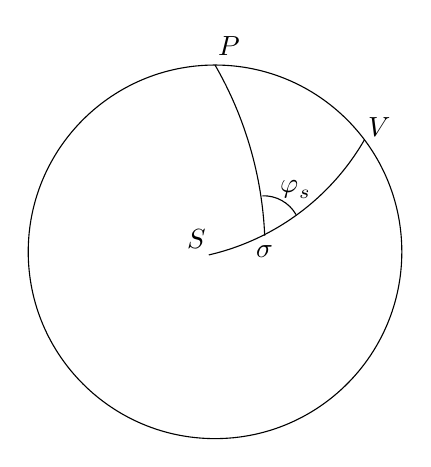
\begin{tikzpicture}[x=0.45pt, y=0.45pt, yscale=0.5, xscale=0.5]
% 天球
\draw (300, 0) arc(0:360:300);
% 三角形
\draw (240, 180) arc(-30:-77:390);
\draw (0, 300) arc(30:2.5:600);
\draw (130, 60) arc(30:92:60);
%Text
\draw (20, 330) node {$P$};
\draw (80, 0) node {$\sigma$};
\draw (260, 200) node {$V$};
\draw (130, 100) node {$\varphi_{s}$};
\draw (-30, 20) node {$S$};
\end{tikzpicture}
\captionsetup{justification=raggedright, singlelinecheck=false}
\caption{视差动。}
\label{视差动。}
\end{figure}

假设太阳的本动速度为 $V_{\odot}\,\unit{km\cdot{}s^{-1}}$, 在一年时间中位移了 $nV_{\odot}\,\unit{km}$, 其中 $n$ 为一年的秒数。此位移会在恒星的自行中表现出来。记恒星视差为 $\pi^{\prime\prime}$, 可以定义一个长期视差
\begin{equation}
h^{\prime\prime}=\frac{nV_{\odot}\,\unit{km}}{r}=\frac{nV_{\odot}\,\unit{km}}{\qty{1}{AU}}\pi^{\prime\prime}=\frac{V_{\odot}\pi^{\prime\prime}}{4.74}.
\end{equation}

显然视差动对天体坐标的影响有与自行类似的形式。延长太阳运动方向在天球上投射出太阳向点 $S$, 赤道坐标 $\left(A, D\right)$. 记 $\overset{\frown}{S\sigma}=\lambda$, 恒星位移在通过 $\overset{\frown}{S\sigma}$ 的大圆上,记恒星位移方向为 $V$. 类似地可定义视差动的方向位置角 $\angle{P\sigma V}=\varphi_{s}$, 如图\ref{视差动。}所示。

视差动 $\mu_{s}$ 在赤经赤纬方向的分解为
\begin{align}
\mu_{s\alpha}&=\mu_{s}\sin{\varphi_{s}}\sec{\delta},\\
\mu_{s\sigma}&=\mu_{s}\cos{\varphi_{s}}.
\end{align}

为了确定 $\mu_{s}$, 考虑太阳本动对切向速度的影响
\begin{equation}
V_{\text{T}}'=V_{\odot}\sin{\lambda},
\end{equation}
根据数值关系 $V_{\text{T}}=4.74\dfrac{\mu}{\pi}$ 可得
\begin{equation}
\mu_{s}=\frac{V_{\odot}\pi\sin{\lambda}}{4.74}=h\sin{\lambda}.
\end{equation}
球面三角形 $\Delta{}PS\sigma$ 中用正弦和五元素公式
\begin{align}
\sin{\lambda}\sin{\varphi_{s}}&=\sin{\left(a-A\right)}\cos{D},\\
\sin{\lambda}\cos{\varphi_{s}}&=-\sin{D}\cos{\delta}+\cos{D}\sin{\delta}\cos{\left(a-A\right)}.
\end{align}
代入得到
\begin{align}
\mu_{s\alpha}&=h\sin{\left(a-A\right)}\cos{D}\sec{\delta},\\
\mu_{s\delta}&=h\left[\cos{D}\sin{\delta}\cos{\left(a-A\right)}-\sin{D}\cos{\delta}\right].
\end{align}
同样太阳本动对视向速度的影响可以表示为
\begin{equation}
V_{r}'=-V_{\odot}\cos{\lambda}=-V_{\odot}\left[\sin{D}\sin{\delta}+\cos{D}\cos{\delta}\cos{\left(a-A\right)}\right].
\end{equation}

\subsubsection{银河系自转}
记 LSR 原点为 $O$, 恒星为 $S$, 银心为 $C$. $O$ 和 $S$ 指向 $C$ 的矢量分别为 $\vec{R}_{0}$ 和 $\vec{R}$, $O$ 指向 $S$ 的矢量为 $r\vec{S}$. 精度允许范围内 $R-R_{0}=-r\cos{b}\cos{l}$.

银河系自转方向和银经增加方向相反,因此可以记天体绕银心公转角速度为
\begin{equation}
\omega=\begin{pmatrix}
0\\
0\\
-\omega
\end{pmatrix}.
\end{equation}
不同半径处角速度不同,可见恒星相对本地静止速度为
\begin{equation}
\vec{v}=\vec{V}-\vec{V}_{0}=\left(\vec{\omega}-\vec{\omega}_{0}\right)\times\vec{R}_{0}+r\vec{\omega}\times\vec{S}.
\end{equation}
由于
\begin{equation}
\vec{S}=\vec{S}\left(l, b\right)=\begin{pmatrix}
\cos{b}\cos{l}\\
\cos{b}\sin{l}\\
\sin{b}
\end{pmatrix},
\end{equation}
可改写成
\begin{equation}
\vec{v}=\begin{pmatrix}
r\omega\sin{l}\cos{b}\\
R_{0}\left(\omega-\omega_{0}\right)-r\omega\cos{l}\cos{b}\\
0
\end{pmatrix},
\end{equation}
因此银河系自转引起的视向速度为
\begin{equation}
v_{r}=\vec{v}\cdot\vec{S}=R_{0}\left(\omega-\omega_{0}\right)\cos{b}\sin{l}.
\end{equation}
$r\ll R_{0}$ 时,有近似表达式
\begin{equation}
\omega-\omega_{0}=\left(\frac{\symup{d}\omega}{\symup{d}R}\right)_{0}\left(R-R_{0}\right).
\end{equation}
定义奥尔特常数,用 $\unit{km\cdot{}s^{-1}\cdot kpc^{-1}}$ 作为单位
\begin{align}
A&=-\frac{1}{2}R_{0}\left(\frac{\symup{d}\omega}{\symup{d}R}\right)_{0},\\
B&=A-\omega_{0}.
\end{align}
结合 $R-R_{0}=-r\cos{b}\cos{l}$ 可得
\begin{align}
R_{0}\left(\omega-\omega_{0}\right)&=2Ar\cos{b}\cos{l},\\
v_{r}&=Ar\cos^{2}{b}\sin{\left(2l\right)}.
\end{align}
其中 $r$ 单位为 $\unit{kpc}$, $v_{r}$ 单位为 $\unit{km\cdot{}s^{-1}}$.

而银河系自转引起的切向速度的银经和银纬分量可分别写为
\begin{align}
v_{l}&=\vec{v}\cdot\vec{l},\\
v_{b}&=\vec{v}\cdot\vec{b}.
\end{align}
$\vec{l}$ 沿着银经增加的方向,因此它平行于银道面并且垂直于 $\vec{S}$, 银河系自转方向与银经增加的方向相反,因此 $\vec{l}$ 与 $-\vec{\omega}\times\vec{S}$ 平行。$\vec{b}$ 沿着银纬增加的方向,垂直于 $\vec{S}$ 和 $\vec{l}$. 因此有
\begin{align}
\vec{l}&=-\frac{\vec{\omega}\times\vec{S}}{\omega\cos{b}}=\begin{pmatrix}
-\sin{l}\\
\cos{l}\\
0
\end{pmatrix},\\
\vec{b}&=\vec{S}\times\vec{l}=-\frac{\vec{S}\times\left(\vec{\omega}\times\vec{S}\right)}{\omega\cos{b}}=\begin{pmatrix}
-\cos{l}\sin{b}\\
\sin{l}\cos{b}\\
\cos{b}
\end{pmatrix}.
\end{align}
代入得到
\begin{align}
v_{l}&=-r\omega\cos{b}+R_{0}\left(\omega-\omega_{0}\right)\cos{l},\\
v_{b}&=-R_{0}\left(\omega-\omega_{0}\right)\sin{l}\sin{b}.
\end{align}

总结:三个方向速度分量
\begin{equation}
\begin{pmatrix}
\vec{V}_{l}\\
\vec{V}_{b}\\
\vec{V}_{r}
\end{pmatrix}=
\begin{pmatrix}
-r\omega\cos{b}+R_{0}\left(\omega-\omega_{0}\right)\cos{l}\\
-R_{0}\left(\omega-\omega_{0}\right)\sin{l}\sin{b}\\
R_{0}\left(\omega-\omega_{0}\right)\sin{l}\cos{b}
\end{pmatrix}.
\end{equation}

还可以写成
\begin{equation}
\begin{cases}
V_{l}=Ar\cos{\left(2l\right)}\cos{b}+Br\cos{b},\\
V_{b}=-Ar\sin{\left(2l\right)}\sin{b}\cos{b},\\
V_{r}=Ar\cos^{2}{b}\sin{\left(2l\right)}.
\end{cases}
\end{equation}
据此得到银经自行 $\mu_{l}$ 和 $\mu_{b}$ 为
\begin{align}
\mu_{l}&=\frac{A}{4.74}\cos{\left(2l\right)}+\frac{B}{4.74},\\
\mu_{b}&=-\frac{A}{4.74}\sin{\left(2l\right)}\sin{b}\cos{b}.
\end{align}
此时自行单位是 $\unit{mas\cdot{}yr^{-1}}$.

要得到对赤经赤纬自行的影响,可以重新分配
\begin{align}
\mu_{\alpha}\cos{\delta}&=\left(\frac{A}{4.74}\cos{\left(2l\right)}\cos{b}+\frac{B}{4.74}\cos{b}\right)\cos{\psi}+\frac{A}{4.74}\sin{\left(2l\right)}\sin{b}\cos{b}\sin{\psi},\\
\mu_{\delta}&=\left(\frac{A}{4.74}\cos{\left(2l\right)}\cos{b}+\frac{B}{4.74}\cos{b}\right)\sin{\psi}-\frac{A}{4.74}\sin{\left(2l\right)}\sin{b}\cos{b}\cos{\psi}.
\end{align}
其中 $\psi$ 是银道星位角。

%\printbibliography

\end{document}